\documentclass[aspectratio=169,11pt,t]{beamer}
% ============================================================
%  ksa-cs-v2: ksa-cs-lecture-template.tex 스타일 + 한글, v2 덱(16:9)용.
%    - 짙은 네이비 헤드라인 (섹션 이름 + 프레임마다 점)
%    - 꽉 찬 파란 제목 막대, 둥근 그림자 블록
%    - 한글: Noto Sans CJK KR (fontspec)
%  사용:
%    \documentclass[aspectratio=169,11pt,t]{beamer}
%    \input{<..>/theme/ksa-cs-v2.tex}
%  ksa-theme.tex 의 매크로(\kb \kq, ksablue/ksared 등)도 같은 이름으로 둔다
%  -> v2 덱 본문을 거의 그대로 옮길 수 있다.
% ============================================================

\usepackage{fontspec}
\usepackage{amsmath,amssymb}
\usepackage{tikz}
\usepackage{listings}
\usepackage{graphicx}
\usepackage{booktabs}
\usepackage{varwidth}
% enumitem 은 넣지 않는다 (beamer 글머리표가 사라진다)

\defaultfontfeatures{Ligatures=TeX}
\setmainfont{Noto Sans CJK KR}
\setsansfont{Noto Sans CJK KR}
\setmonofont{Noto Sans Mono CJK KR}[Scale=0.92]
\usefonttheme{professionalfonts}

% ---------- 기본 틀 ----------
\usetheme{default}
\useinnertheme[shadow=true]{rounded}
\setbeamertemplate{navigation symbols}{}
\setbeamersize{text margin left=1em,text margin right=1em}

% ---------- 색 (템플릿 원본 값) ----------
\definecolor{navydark}{HTML}{191959}
\definecolor{navydim}{HTML}{8888B0}
\definecolor{navytitle}{HTML}{262686}
\definecolor{navyblue}{HTML}{3333B2}
\definecolor{blockbodybg}{HTML}{E9E9F3}
\definecolor{examplegreen}{HTML}{006000}
\definecolor{examplebg}{HTML}{E5EFE5}
\definecolor{alertred}{HTML}{BF0000}
\definecolor{alertbg}{HTML}{F9E5E5}
% ksa-theme.tex 와 같은 이름 (본문 호환)
\colorlet{ksablue}{navytitle}
\colorlet{ksabluedk}{navydark}
\definecolor{ksagold}{HTML}{D6CBB1}
\definecolor{ksagolddk}{HTML}{A9976B}
\colorlet{ksared}{alertred}
\definecolor{ksagray}{HTML}{5B5B5B}

\setbeamercolor{structure}{fg=navyblue}
\setbeamercolor{alerted text}{fg=alertred}
\setbeamercolor{frametitle}{bg=navytitle,fg=white}
\setbeamercolor{title}{fg=white,bg=navytitle}
\setbeamercolor{block title}{bg=navytitle,fg=white}
\setbeamercolor{block body}{bg=blockbodybg,fg=black}
\setbeamercolor{block title example}{bg=examplegreen,fg=white}
\setbeamercolor{block body example}{bg=examplebg,fg=black}
\setbeamercolor{block title alerted}{bg=alertred,fg=white}
\setbeamercolor{block body alerted}{bg=alertbg,fg=black}
\setbeamercolor{item}{fg=navyblue}
\setbeamertemplate{itemize item}[circle]
\setbeamertemplate{itemize subitem}[triangle]

% ---------- 헤드라인: miniframes (섹션 이름 + 점) ----------
\useoutertheme[subsection=false]{miniframes}
\setbeamerfont{section in head/foot}{size=\tiny}
\setbeamercolor{section in head/foot}{bg=navydark,fg=white}
\setbeamercolor{mini frame}{fg=white}
\setbeamertemplate{mini frames}[circle]

% ---------- 제목 막대: 폭 꽉 채움, 두 줄까지 ----------
\setbeamerfont{frametitle}{size=\normalsize,series=\bfseries}
\setbeamertemplate{frametitle}{%
  \nointerlineskip
  \begin{beamercolorbox}[wd=\paperwidth,ht=2.7ex,dp=1.1ex,leftskip=.3cm,rightskip=.3cm]{frametitle}%
    \usebeamerfont{frametitle}\insertframetitle
  \end{beamercolorbox}}

% ---------- 쪽 번호: 오른쪽 아래 ----------
\setbeamertemplate{footline}{%
  \hfill
  {\color{navydim}\scriptsize\insertframenumber\,/\,\inserttotalframenumber}%
  \hspace{3mm}\vspace{2mm}%
}

% ---------- 표지: 템플릿처럼 헤드라인은 그대로, 가운데 둥근 그림자 상자에 제목 한 줄 ----------
% 덱에서:  {\setbeamertemplate{footline}{}\begin{frame}[c,noframenumbering]\titlepage\end{frame}}
\setbeamercolor{title}{fg=white,bg=navyblue}
\makeatletter
\setbeamertemplate{title page}{%
  \vfill
  \centering
  \begin{minipage}{0.84\paperwidth}
  \begin{beamercolorbox}[wd=\linewidth,sep=7pt,center,rounded=true,shadow=true]{title}
    {\usebeamerfont{title}\inserttitle\par}%
    \ifx\insertsubtitle\@empty\else\vskip0.4em{\usebeamerfont{subtitle}\insertsubtitle\par}\fi
  \end{beamercolorbox}
  \end{minipage}\par\vskip1.6em
  {\usebeamerfont{author}\color{navytitle}\insertauthor\par}\ifx\beamer@date\@empty\vskip0.3em\else\vskip1.3em\fi
  {\usebeamerfont{institute}\color{ksagray}\insertinstitute\par}%
  \ifx\beamer@date\@empty\else\vskip0.3em{\usebeamerfont{date}\color{ksagray}\insertdate\par}\fi
  \vfill
}
\makeatother
\setbeamerfont{title}{series=\bfseries,size=\Large}
\setbeamerfont{subtitle}{size=\normalsize}
\setbeamerfont{author}{size=\normalsize}
\setbeamerfont{institute}{size=\small}
\setbeamerfont{date}{size=\small}

% ksa-theme 호환: 덱이 \renewcommand{\ksacredit}{..} 를 해도 되게 (꼬리말에는 안 쓴다)
\newcommand{\ksacredit}{}

% ---------- 강조 ----------
\newcommand{\hl}[1]{\textcolor{alertred}{#1}}
\newcommand{\hlb}[1]{\textcolor{navyblue}{#1}}
\newcommand{\kb}[1]{\textbf{\color{ksablue}#1}}
\newcommand{\kq}[1]{\textbf{\color{ksared}#1}}

% ---------- 파이썬 코드 (템플릿과 같은 색) ----------
\definecolor{codekw}{HTML}{0033B3}
\definecolor{codebuiltin}{HTML}{BF0000}
\definecolor{codestr}{HTML}{067D17}
\definecolor{codecomment}{HTML}{8C8C8C}
\definecolor{codenum}{HTML}{1750EB}
\lstdefinestyle{py}{
  language=Python, basicstyle=\ttfamily\scriptsize,
  keywordstyle=\color{codekw}\bfseries, stringstyle=\color{codestr},
  commentstyle=\color{codecomment}\itshape, numberstyle=\color{codenum},
  emph={print,len,range,sum,input,int,str,float,list,dict,append,remove,sorted,abs,min,max},
  emphstyle=\color{codebuiltin}, showstringspaces=false, keepspaces=true,
  columns=fixed, basewidth=0.52em, aboveskip=1mm, belowskip=1mm, xleftmargin=2mm,
  breaklines=true
}
\lstset{style=py}

\usepackage{fontawesome5}
\newcommand{\paperlink}[1]{\href{#1}{\textcolor{ksablue}{\faLink}}}
% SVM 수업 두 덱 중 첫째 (2026-11-26 Stanford CME 250 범위로: 학습 과정·크기 약속·라그랑주는 보충 덱 ../9_svm_extra)
\setbeamerfont{author}{size=\normalsize}
\setbeamerfont{institute}{size=\small}
\graphicspath{{figs/}{../../../assets/}}
\usetikzlibrary{tikzmark,shapes.callouts,positioning}
\tikzset{bub/.style={draw=ksagolddk,line width=1pt,fill=ksagolddk!10,rounded corners=3pt,inner sep=4pt,font=\normalsize,align=left},
         bubarr/.style={-latex,ksagolddk,line width=1.2pt}}
\definecolor{fgap}{HTML}{1B7F3B}\definecolor{fx}{HTML}{D62728}\definecolor{fsh}{HTML}{2E3192}\definecolor{fbeta}{HTML}{7A6A3F}\definecolor{fdist}{HTML}{000000}\definecolor{fbd}{HTML}{555555}
\makeatletter
\newcommand{\markpage}[1]{\protected@write\@auxout{}{\string\newlabel{#1}{{\the\c@framenumber}{}}}\hypertarget{#1}{}}
\newcommand{\pref}[1]{\hyperlink{#1}{\textcolor{ksagolddk}{(p.\ref{#1})}}}
\makeatother

\renewcommand{\ksacredit}{Machine Learning and Deep Learning \,\textperiodcentered\, SVM 1: 최대 마진 · 소프트 마진}
\title{SVM 1: 최대 마진 · 소프트 마진 (Support Vector Machine)}
\subtitle{초평면 · 최대 마진 · 소프트 마진}
\author{Machine Learning and Deep Learning}
\institute{KSA 2027-Spring}
\date{Sumin Han (suminhan@ksa.hs.kr)}
\begin{document}
{\setbeamertemplate{footline}{}\begin{frame}[c,noframenumbering]\titlepage\end{frame}}

\section{질문}
% --- 오늘의 질문
\begin{frame}{오늘의 질문}
\vfill
\begin{columns}[c]
\begin{column}{0.44\textwidth}\centering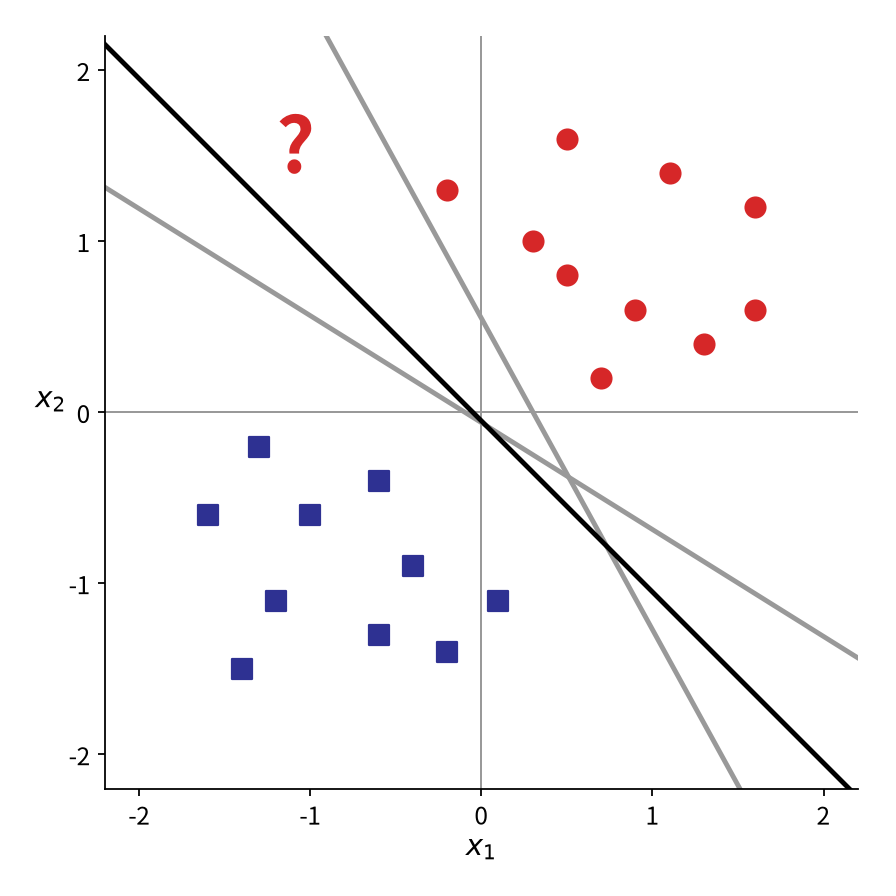
\includegraphics[width=0.95\linewidth]{sv_hook.png}\end{column}
\begin{column}{0.52\textwidth}
{\large 세 선 모두 \textbf{완벽하게} 가른다}\\[0.8em]
{\Large \kq{어느 선이 가장 좋을까?}}
\end{column}
\end{columns}
\vfill
\note{빨간 점과 파란 점이 있습니다. 둘을 가르는 직선을 세 개 그었는데, 세 선 모두 학습 데이터를 하나도 틀리지 않고 완벽하게 가릅니다. 학습 오차로는 셋 다 0입니다. 그런데 어느 선이 가장 좋을까요? 직관적으로는 가운데 검은 선이 가장 안심이 됩니다. 왜 그런지, 그리고 그 선을 어떻게 찾는지가 오늘의 주제입니다.}
\end{frame}

% --- 데이터는 먼저 z-score
\begin{frame}{먼저: 점들은 z-score normalization 해 둔다}
\vfill
\centering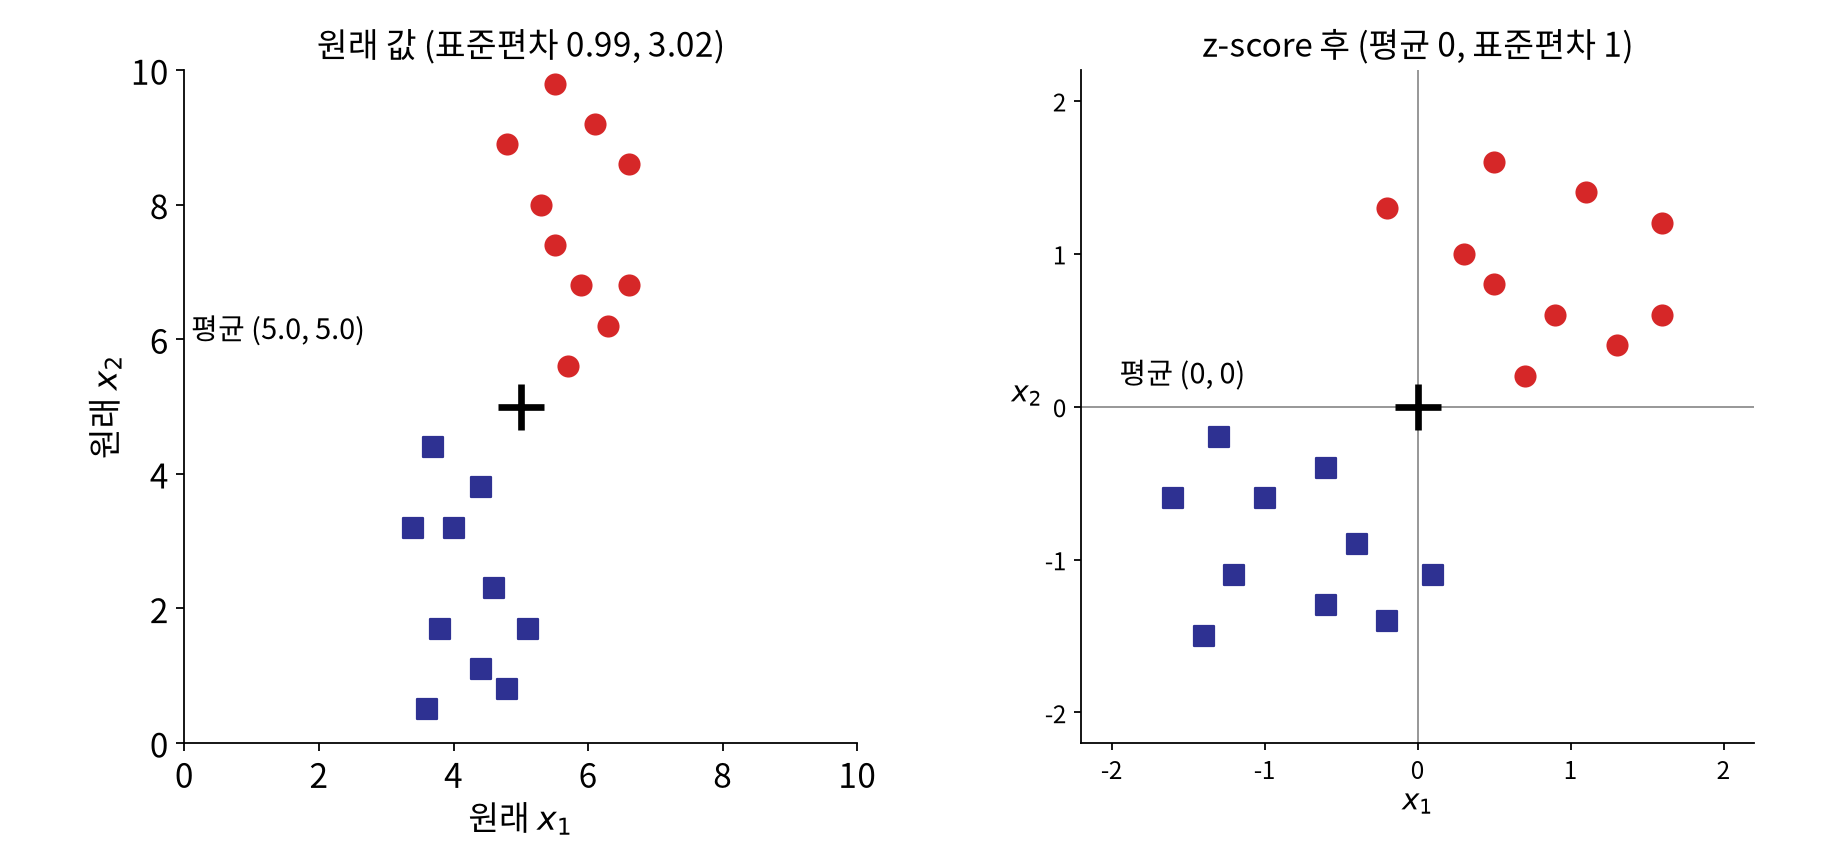
\includegraphics[width=0.8\linewidth]{sv_raw_z.png}\par\vskip0.2em
{\large $z = (x - \text{평균}) / \text{표준편차}$ \quad (축마다) \quad 이 덱의 점은 모두 \kb{z-score 한 값}}
\vfill
\note{시작하기 전에 데이터를 한 번 손봅니다. 왼쪽이 원래 값입니다. 각 축에서 평균을 빼고 표준편차로 나누면 오른쪽처럼 점들이 원점 주변에 크기 1 정도로 모입니다. 이것을 z-score라고 합니다. x1은 평균 5, 표준편차 약 1이고, x2는 평균 5, 표준편차 약 3입니다. 세로로 3배 더 퍼져 있던 것이 z-score 후에는 두 축 모두 크기 1로 맞춰집니다. 오늘 덱의 점 20개, 그림, 숫자는 모두 이 z-score 한 값입니다. 소수 첫째 자리로 반올림했습니다. 모양은 그대로이고 눈금만 바뀝니다. 왜 이렇게 하는지는 학습 부분에서 봅니다. 하지 않으면 학습이 아예 실패할 수 있습니다. sklearn으로 SVM을 쓸 때도 StandardScaler로 z-score를 먼저 하는 것이 기본입니다.}
\end{frame}

% --- 파랑 뒤집기 → 평균 (한 쪽에 세 장)
\begin{frame}{가장 쉬운 방법: 점에 $y_k$ 를 곱해 평균 내기}
\markpage{meanvec}
\vfill
\centering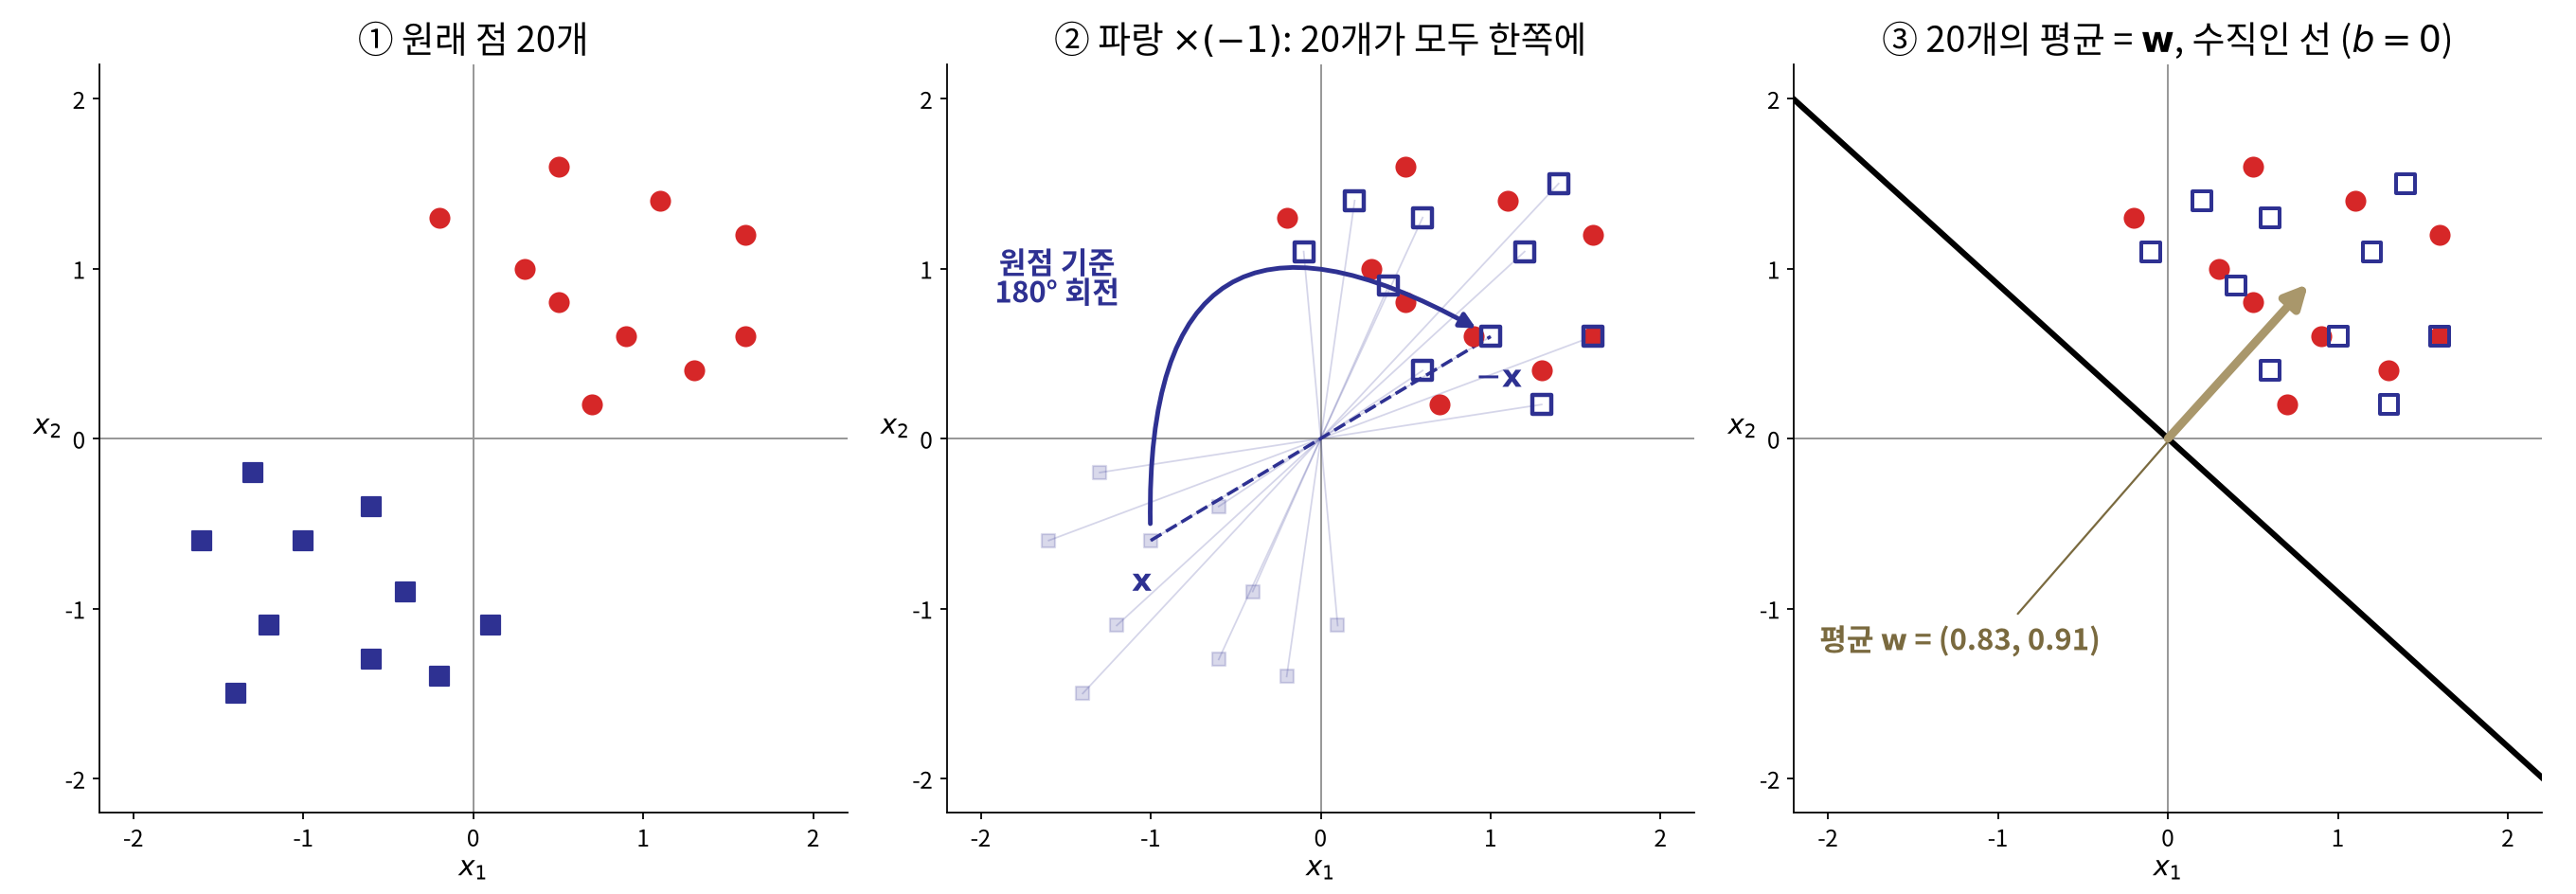
\includegraphics[width=\linewidth]{sv_flip_mean.png}\par\vskip0.2em
{\large 파랑은 \kb{원점 기준 180° 회전} \;$\to$\; $\mathbf{w} = \dfrac{1}{p}\sum_{k=1}^{p} y_k\mathbf{x}_k = (0.83,\ 0.91)$, \;$b = 0$}
\vfill
\note{가장 먼저 떠오르는 방법부터 해 봅시다. 세 그림을 왼쪽부터 차례로 봅니다. 첫째 그림은 원래 점 20개입니다. 둘째 그림, 파란 점의 좌표 두 개에 모두 마이너스를 붙입니다. 라벨 y가 파랑은 마이너스 1이니, y k 곱하기 x k입니다. 좌표 두 개의 부호를 모두 바꾸면 원점을 중심으로 180도 돌린 것, 점대칭입니다. 선을 거울로 비추는 대칭이 아닙니다. 예를 들어 파란 점 마이너스 1, 마이너스 0.6은 1, 0.6으로 갑니다. 빈 네모가 뒤집은 파란 점이고, 이제 20개가 모두 빨강 쪽, 한쪽에 모입니다. 셋째 그림, 원점에서 각 점까지의 화살표, 즉 벡터 20개의 평균을 내면 금색 화살표, 0.83, 0.91입니다. 이 화살표를 w로 쓰고, w에 수직이고 원점을 지나는 선을 긋습니다. 점들을 z-score 해서 가운데가 원점이니 b는 0으로 둡니다. 계산은 평균 한 번이면 끝납니다. 뒤에서 나오는 거울로 접기는 경계를 거울 삼는 것이라 다른 이야기입니다. 그리고 뒤에서 보겠지만 이 선은 SVM 학습의 1걸음 뒤 첫 선과 똑같습니다.}
\end{frame}

% --- 다듬기: 평균 선 vs SVM
\begin{frame}{SVM: 가장 가까운 점 기준으로 다듬는다}
\vfill
\centering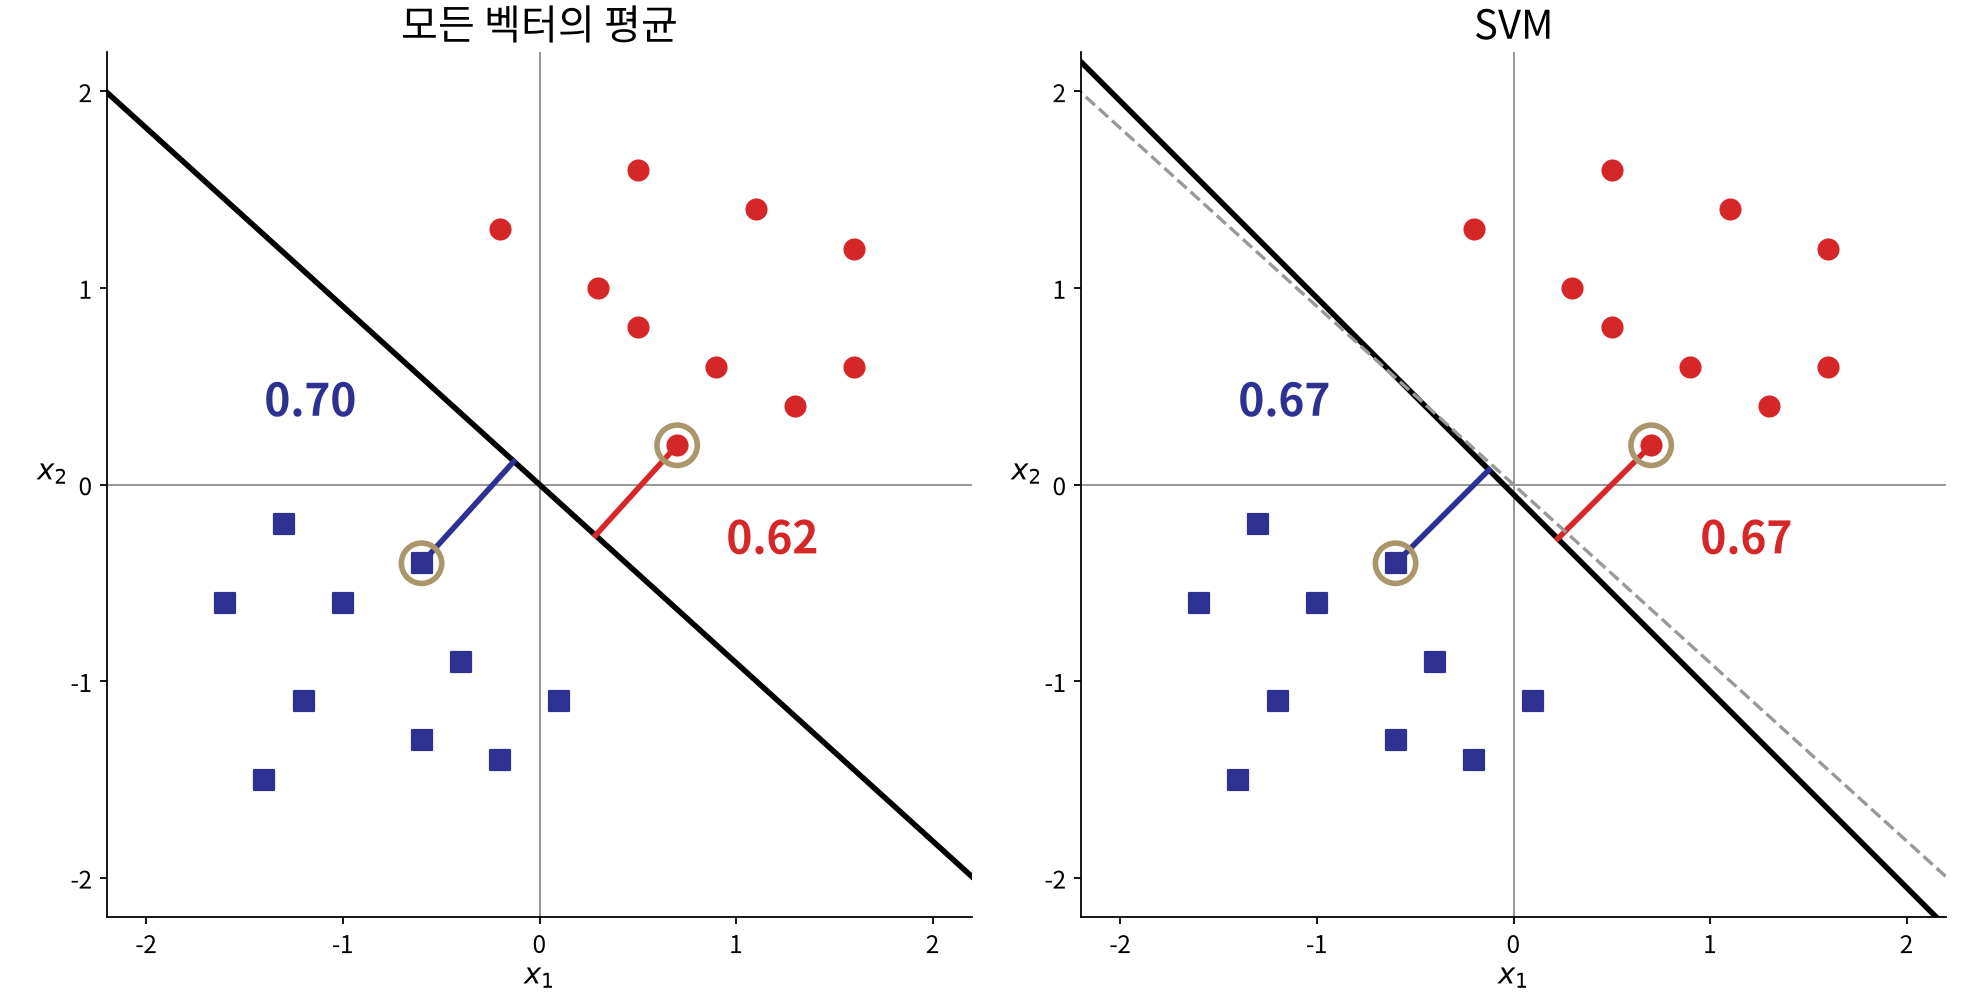
\includegraphics[width=0.78\linewidth]{sv_centroid_vs.png}\par\vskip0.2em
{\large 평균 선: 빨강 쪽으로 \kq{치우침} (0.62 vs 0.70) \quad SVM: 양쪽 \kb{0.67}}
\vfill
\note{그런데 이 평균 선에서 가장 가까운 점까지 거리를 재 보면, 빨간 점 0.7, 0.2까지는 0.62, 파란 점 마이너스 0.6, 마이너스 0.4까지는 0.70입니다. 평균은 먼 점까지 모두 섞어서 정하니, 경계 가까이 있는 점 기준으로 보면 한쪽으로 치우쳐 있습니다. SVM은 평균 대신 경계에 가장 가까운 점들만 보고, 그 사이의 한가운데로 선을 옮깁니다. 그러면 양쪽 모두 0.67로 같아지고, 이것이 가장 가까운 점까지 거리를 가장 크게 만든 선입니다. 회색 점선이 평균 선, 검은 선이 SVM입니다. 뒤에서 볼 학습은 0에서 출발하면 첫 걸음이 바로 이 평균 선이 되고, 그 뒤 가장 가까운 점들이 밀면서 SVM 선으로 다듬어 갑니다.}
\end{frame}

% --- 로지스틱회귀 vs SVM
\begin{frame}{로지스틱회귀 vs SVM}
\vfill
\centering
\renewcommand{\arraystretch}{2.2}
{\LARGE\begin{tabular}{l|l}
로지스틱회귀 & \textbf{모든 점}이 선을 민다 (틀릴수록 세게)\\ \hline
\kb{SVM} & \kb{가장 가까운 점}만 선을 민다
\end{tabular}}\\[1.2em]
{\large 값 계산은 둘 다 \textbf{모든 점}에 대해 한다}
\vfill
\note{세 방법을 학습 한 걸음으로 비교합니다. 세 방법 모두 한 걸음은 같은 꼴입니다. w에 학습률 곱하기 색 곱하기 좌표를 더하는데, 점마다 그 점이 미는 세기를 곱합니다. 다른 것은 이 세기뿐입니다. 모든 점의 평균 선은 모든 점이 똑같이 1로 밉니다. 먼 점도 가까운 점도 같은 무게입니다. 로지스틱회귀는 시그모이드로 계산한 틀릴 확률만큼 밉니다. 경계에서 멀고 맞는 점은 틀릴 확률이 0에 가까워 거의 안 밀고, 경계 근처는 0.5쯤, 틀린 점은 1에 가깝게 세게 밉니다. 다만 먼 점도 0은 아니라서 아주 조금씩은 계속 밉니다. 로지스틱 손실, 크로스 엔트로피를 미분하면 바로 이 꼴이 나옵니다. SVM도 가장 가까운 점을 찾으려면 매 걸음 20개 점의 값을 모두 계산해야 합니다. 계산은 모두 하고, 그중 값이 가장 작은 점, 즉 경계에 가장 가까운 점만 밀고 나머지는 미는 세기가 정확히 0입니다. 그래서 학습이 끝나면 가장 가까운 점 몇 개, 서포트 벡터만 남습니다. 시험으로 치면 로지스틱은 이미 잘하는 학생은 거의 안 세고 못하는 학생일수록 크게 세는 평균, SVM은 그 거의 안 셈을 아예 안 셈으로 끊어 꼴찌 몇 명만 보는 것입니다.}
\end{frame}

% --- 원 논문
\begin{frame}{SVM 의 원 논문}
\vfill
\centering
\renewcommand{\arraystretch}{1.9}
{\large\begin{tabular}{c@{\hspace{1em}}p{5.3cm}l}
\textbf{1992} & Boser, Guyon, Vapnik & \kb{최대 마진} 학습 + \kb{커널}\\[-0.4em]
 & \multicolumn{2}{l}{\small \textit{A training algorithm for optimal margin classifiers} (COLT '92) \paperlink{https://doi.org/10.1145/130385.130401}}\\[0.6em]
\textbf{1995} & Cortes, Vapnik & \kb{소프트 마진}, ``Support Vector'' 라는 이름\\[-0.4em]
 & \multicolumn{2}{l}{\small \textit{Support-vector networks} (\textit{Machine Learning} 20(3)) \paperlink{https://doi.org/10.1007/BF00994018}}
\end{tabular}}\\[1.2em]
{\large 덱의 기호 ($D(\mathbf{x})$, $M$, $y_k$ · 다음 시간 $\alpha_k$, $\xi_k$, $C$) 는 \kb{두 논문 그대로}}
\vfill
\note{오늘 배울 서포트 벡터 머신이 어디서 왔는지부터 봅시다. 원 논문은 보통 두 편을 같이 꼽습니다. 첫째는 1992년, AT&T 벨 연구소의 Guyon과 Vapnik, 그리고 Boser가 COLT라는 학회에 낸 A training algorithm for optimal margin classifiers입니다. 경계와 가장 가까운 점 사이의 여백, 마진을 가장 크게 하는 학습법을 내고, 커널을 써서 직선이 아닌 휘어진 경계까지 같은 방법으로 학습할 수 있다는 것을 보였습니다. 오늘 배우는 최대 마진과 세 번째 시간의 커널이 이 논문입니다. 최대 마진으로 직선을 고르는 생각 자체는 1960년대 Vapnik의 generalized portrait 방법까지 거슬러 올라가고, 커널로 점곱을 바꾸는 생각도 1964년 Aizerman 등의 논문에 있었습니다. 이 논문은 둘을 합쳤습니다. 둘째는 1995년 Cortes와 Vapnik이 Machine Learning 저널에 낸 Support-vector networks입니다. 1992년 논문은 두 무리가 직선으로 깔끔하게 갈릴 때만 다뤘는데, 이 논문이 몇 점은 넘어가도 되는 소프트 마진을 더해 실제 데이터에 쓸 수 있게 했고, 서포트 벡터라는 이름도 이 논문 제목에서 나왔습니다. 두 논문 모두 손글씨 숫자 인식으로 실험했습니다. 이 덱의 기호는 두 논문을 그대로 따릅니다. 결정 함수 D, 마진 대문자 M, 점 번호 k와 라벨 y k는 1992년 논문, 슬랙 크사이와 벌점 C는 1995년 논문 기호입니다.}
\end{frame}

% --- 비하인드
\begin{frame}{비하인드: AT\&T 벨 연구소, 1990년대 초}
\vfill
\centering
\renewcommand{\arraystretch}{1.45}
{\large\begin{tabular}{rl}
\textbf{커널은 누구 생각?} & Vapnik: ``특징을 곱해서 늘리자'' $\to$ Guyon: ``\kb{커널}로 하자''\\[0.8em]
\textbf{1995년 내기} & 신경망은 잘 맞히는데 \kq{왜 되는지 이론이 없던} 때\\
 & Jackel: ``2000년까지 \kb{이유를 알게 된다}''\\[-0.3em]
 & \hspace*{1.5em}{\normalsize $\to$ \kq{틀림}: 지금도 다 못 풀었다}\\
 & Vapnik: ``2005년엔 신경망이 \kb{안 쓰인다}''\\[-0.3em]
 & \hspace*{1.5em}{\normalsize $\to$ \kq{틀림}: 지금 가장 많이 쓰는 모델이 됐다}
\end{tabular}}\\[1.2em]
{\large 결과: \kq{둘 다 졌다}}
\vfill
\note{비하인드 이야기 두 개입니다. SVM은 1990년대 초 미국 AT&T 벨 연구소에서 나왔습니다. Vapnik은 소련에서 1960년대부터 학습 이론을 연구하다가 1990년에 미국으로 건너와 이 연구소에 합류했습니다. 첫째, 커널은 누구 생각이었을까요. 1992년 논문의 저자인 Isabelle Guyon이 2016년에 직접 쓴 회고에 따르면, 직선을 긋는 최대 마진 학습이 먼저 잘 되자, Vapnik은 특징끼리 곱해서 특징을 늘리자고 했고, Guyon은 대신 예전 potential function 방법의 커널 트릭을 쓰자고 했다고 합니다. 세 번째 시간에 배울 바로 그 커널입니다. Guyon은 Vapnik과 사무실을 같이 쓰며 열띤 토론을 했다고 적었고, 1저자 Bernhard Boser는 Guyon의 남편입니다. 다만 이것은 본인 회고라, 다른 사람의 기억과 다를 수 있습니다. 둘째, 1995년 같은 연구소에서 유명한 내기가 있었습니다. 그때 신경망은 숫자 인식도 잘했지만 왜 잘 되는지 설명하는 이론은 없었습니다. 연구소 그룹장 Larry Jackel은 5년 안에, 2000년까지는 그 이유를 알게 될 것이라고 걸었습니다. 증명되는 이론을 중시한 Vapnik은 이유도 모르는 큰 신경망은 2005년이면 아무도 역전파로 학습하지 않을 것이라고 걸었습니다. Yann LeCun도 같은 연구소에 있었고, Geoffrey Hinton이 강의에서 이 내기 문서를 소개한 적이 있습니다. 결과는 둘 다 졌습니다. Jackel이 건 것처럼 2000년까지 이유를 알아내지 못했고, Vapnik이 건 것처럼 신경망이 사라지지도 않았습니다. 신경망이 왜 그렇게 잘 되는지는 아직도 다 풀리지 않았고, 신경망은 지금 가장 많이 쓰는 모델이 됐습니다. 그래도 SVM은 2000년대 내내 가장 많이 쓰인 분류기 중 하나였고, 답이 하나로 정해지고 이론이 깔끔해서 지금도 데이터가 아주 크지 않을 때 많이 씁니다. 10년 뒤 2014년에는 Vapnik이 LeCun이 이끄는 페이스북 AI 연구소에 합류했습니다.}
\end{frame}

\section{초평면}
% --- 초평면
\begin{frame}{초평면 (hyperplane): 공간을 반으로 가르는 평평한 면}
\vfill
\centering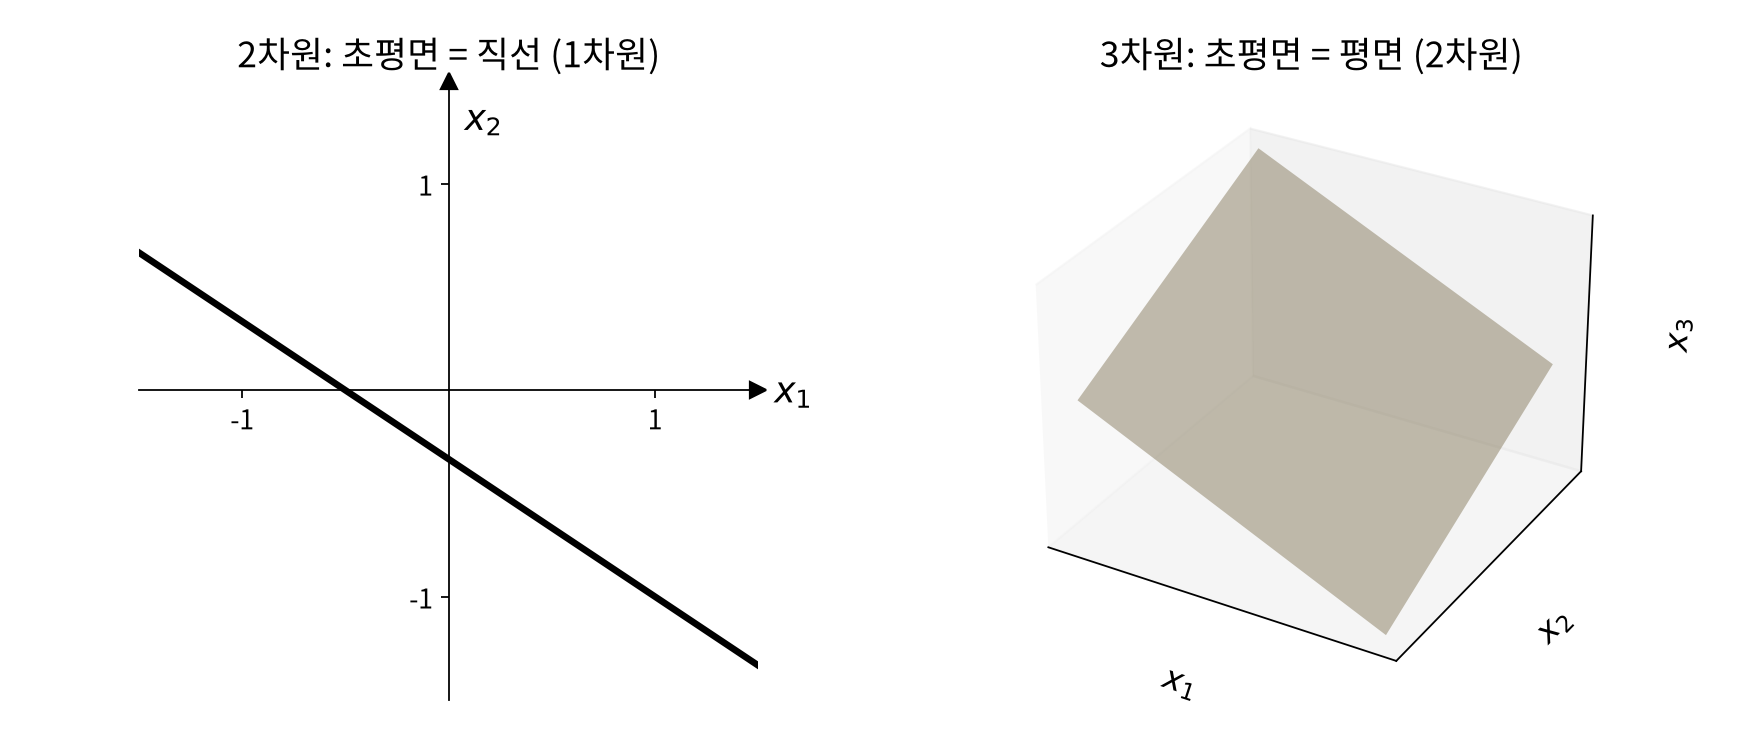
\includegraphics[width=0.78\linewidth]{sv_hyper.png}\par\vskip0.3em
{\large 2차원이면 \kb{직선}, 3차원이면 \kb{평면}}
\vfill
\note{SVM은 초평면이라는 말에서 출발합니다. n차원 공간에서 초평면은 한 차원 낮은, 평평한 면입니다. 특징이 두 개인 2차원 평면에서는 직선이고, 특징이 세 개인 3차원 공간에서는 평면입니다. 특징이 더 많아져도 이름은 그대로 초평면입니다. 오늘은 그림을 그릴 수 있게 대부분 2차원, 즉 직선으로 보겠습니다.}
\end{frame}

% --- 초평면 식
\begin{frame}{초평면의 식: 값이 0 인 곳, 부호로 양쪽을 나눈다}
\vfill
\begin{columns}[c]
\begin{column}{0.44\textwidth}\centering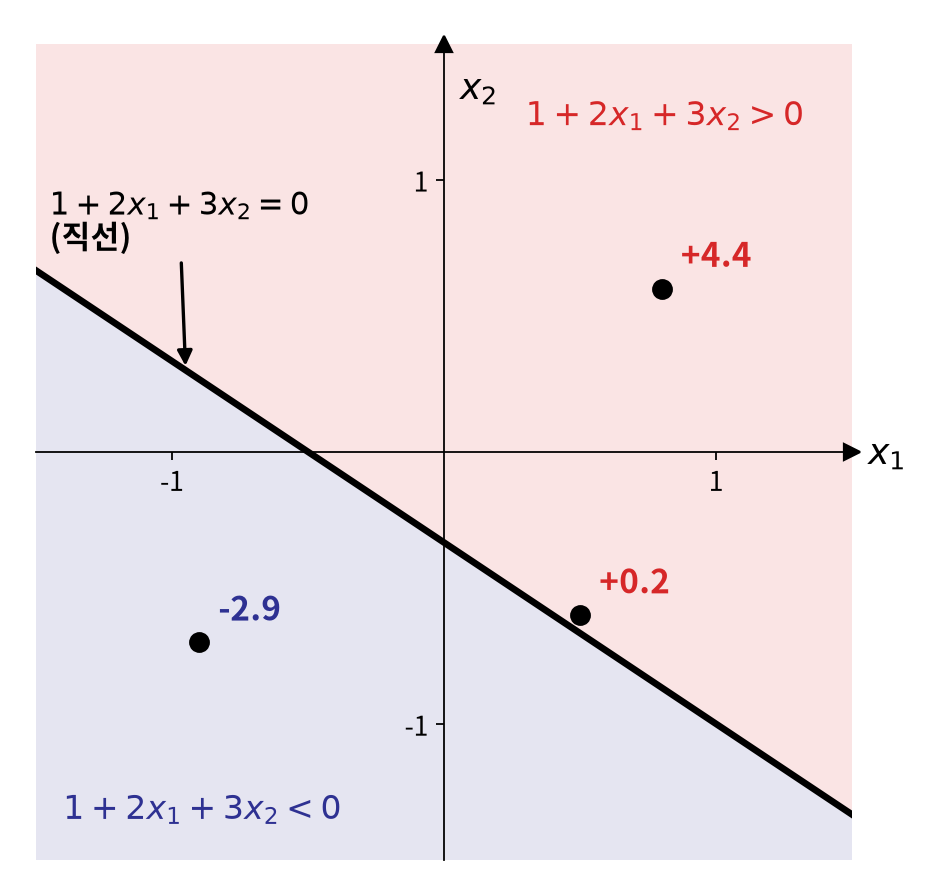
\includegraphics[width=0.92\linewidth]{sv_half.png}\end{column}
\begin{column}{0.54\textwidth}
{\Large $w_1 x_1 + w_2 x_2 + b = 0$}\\[0.8em]
{\large 값 \textcolor{ksared}{$> 0$} 한쪽, \textcolor{ksablue}{$< 0$} 다른 쪽}\\[0.8em]
\begin{itemize}\large
\item 예: $1 + 2x_1 + 3x_2 = 0$
\begin{itemize}\normalsize
\item $(0.8, 0.6) \to \textcolor{ksared}{+4.4}$
\item $(-0.9, -0.7) \to \textcolor{ksablue}{-2.9}$
\end{itemize}
\end{itemize}
\end{column}
\end{columns}
\vfill
\note{2차원 초평면, 직선은 w1 x1 더하기 w2 x2 더하기 b가 0인 점들의 모임입니다. 예를 들어 1 더하기 2 x1 더하기 3 x2가 0인 직선을 그리면 왼쪽 검은 선입니다. 이 직선 위에 있지 않은 점을 넣으면 값이 0이 아니게 나오는데, 한쪽은 모두 양수, 다른 쪽은 모두 음수입니다. 점 0.8, 0.6을 넣으면 플러스 4.4, 점 마이너스 0.9, 마이너스 0.7은 마이너스 2.9입니다. 경계 가까이 있는 점은 0.2처럼 0에 가깝습니다. 그래서 초평면 하나가 공간을 반으로 나누고, 값의 부호만 보면 어느 쪽인지 압니다. 특징이 n개면 항이 n개로 늘어날 뿐 같습니다.}
\end{frame}

% --- 분리 초평면 분류기
\begin{frame}{분리 초평면으로 분류하기}
\vfill
\begin{columns}[c]
\begin{column}{0.36\textwidth}\centering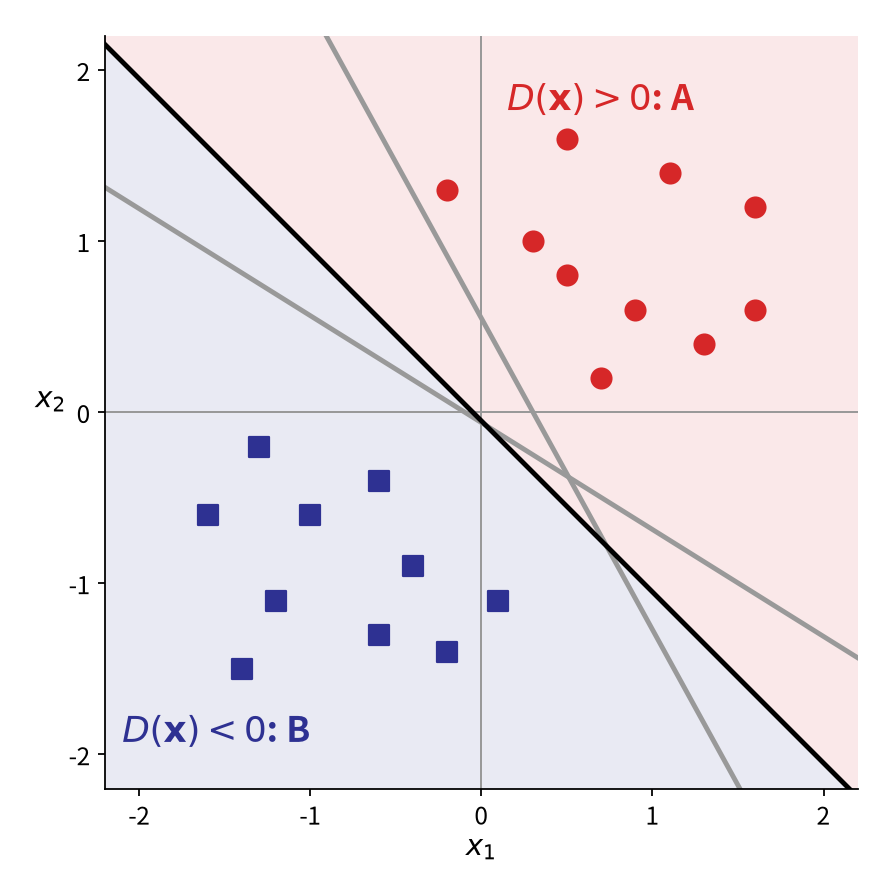
\includegraphics[width=\linewidth]{sv_hook_d.png}\end{column}
\begin{column}{0.63\textwidth}
{\normalsize 학습 데이터 \; $(\mathbf{x}_1, y_1),\ \dots,\ (\mathbf{x}_p, y_p)$, \;$p = 20$}\\[0.2em]
{\normalsize $y_k = \begin{cases} +1 & \mathbf{x}_k \in \text{클래스 A (빨강)}\\ -1 & \mathbf{x}_k \in \text{클래스 B (파랑)} \end{cases}$}\\[0.5em]
{\large $D(\mathbf{x}) = \mathbf{w}\cdot\mathbf{x} + b = \sum_{i=1}^{n} w_i x_i + b$}\\[0.2em]
{\normalsize 분류: $D(\mathbf{x}) > 0$ 이면 A, 아니면 B}\\[0.5em]
{\normalsize 모든 점이 제 색 영역에 \;$\Leftrightarrow$\; \kb{$y_k\, D(\mathbf{x}_k) > 0$}}\\[0.2em]
{\normalsize 그런 선은 검은 선 · 회색 선처럼 \kq{무수히} 많다}
\end{column}
\end{columns}
\vfill
\note{이제 문제를 원 논문처럼 적어 봅시다. 학습 데이터는 점과 라벨의 짝 p개, 여기서는 20개입니다. 점 x k가 클래스 A, 빨강이면 라벨 y k는 플러스 1, 클래스 B, 파랑이면 마이너스 1입니다. 그리고 초평면의 식 w 점곱 x 더하기 b를 D라고 씁니다. SVM 원 논문, Boser, Guyon, Vapnik의 1992년 논문이 쓰는 이름이고, 결정 함수라는 뜻의 decision function에서 왔습니다. 빨간 점에서 D가 양수, 파란 점에서 음수면 잘 가른 것입니다. 두 조건을 한 줄로 쓰면, 라벨 곱하기 D가 모든 점에서 0보다 크다입니다. 라벨이 마이너스 1이면 음수 곱하기 음수라 양수가 되니까요. 새 점이 오면 D가 0보다 크면 A, 아니면 B로 분류하고, D의 절댓값이 클수록, 즉 경계에서 멀수록 더 확신합니다. 로지스틱회귀의 z가 0인 경계도 이런 분리 초평면입니다. 문제는 데이터가 깔끔하게 나뉘면 가르는 선이 그림처럼 무수히 많다는 것입니다. 어느 것을 골라야 할까요.}
\end{frame}

\section{최대 마진}
% --- 가장 넓은 길
\begin{frame}{최대 마진 분류기: 가장 넓은 길}
\markpage{street}
\vfill
\begin{columns}[c]
\begin{column}{0.44\textwidth}\centering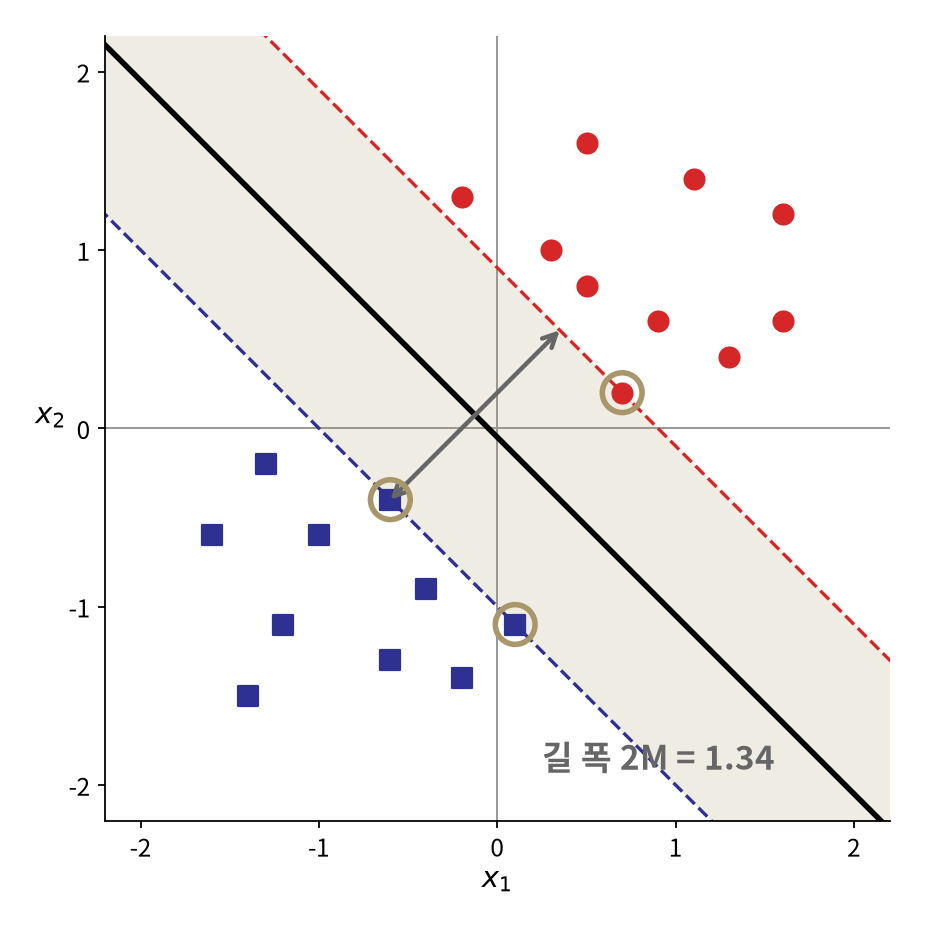
\includegraphics[width=0.95\linewidth]{sv_street.png}\end{column}
\begin{column}{0.52\textwidth}
{\large \kb{마진 $M \in \mathbb{R}$} = 가장 가까운 점까지 거리}\\[0.8em]
{\large $M$ 이 가장 큰 선 = 길의 가운데}\\[0.8em]
{\large $M =$ \kb{0.67} \quad 동그라미 = \textbf{서포트 벡터}}
\end{column}
\end{columns}
\vfill
\note{가장 자연스러운 선택은 양쪽 점에서 가장 멀리 떨어진 초평면입니다. 경계에서 가장 가까운 학습 점까지의 거리를 마진, 대문자 M이라고 부르고, 마진이 가장 큰 초평면을 최대 마진 초평면, 이것으로 분류하는 것을 최대 마진 분류기라고 합니다. 그림으로는 두 무리 사이에 점이 하나도 없는 가장 넓은 길을 내고 그 가운데 선을 경계로 쓰는 것입니다. 이 데이터에서 M은 0.67, 길 전체 폭은 그 두 배인 1.34입니다. 경계까지의 거리가 정확히 M인 점, 점선에 닿은 노란 동그라미 점들을 서포트 벡터라고 부릅니다.}
\end{frame}

% --- 서포트 벡터만
\begin{frame}{왜 ``서포트 벡터'' 인가: 이 점들만 경계를 받친다}
\vfill
\centering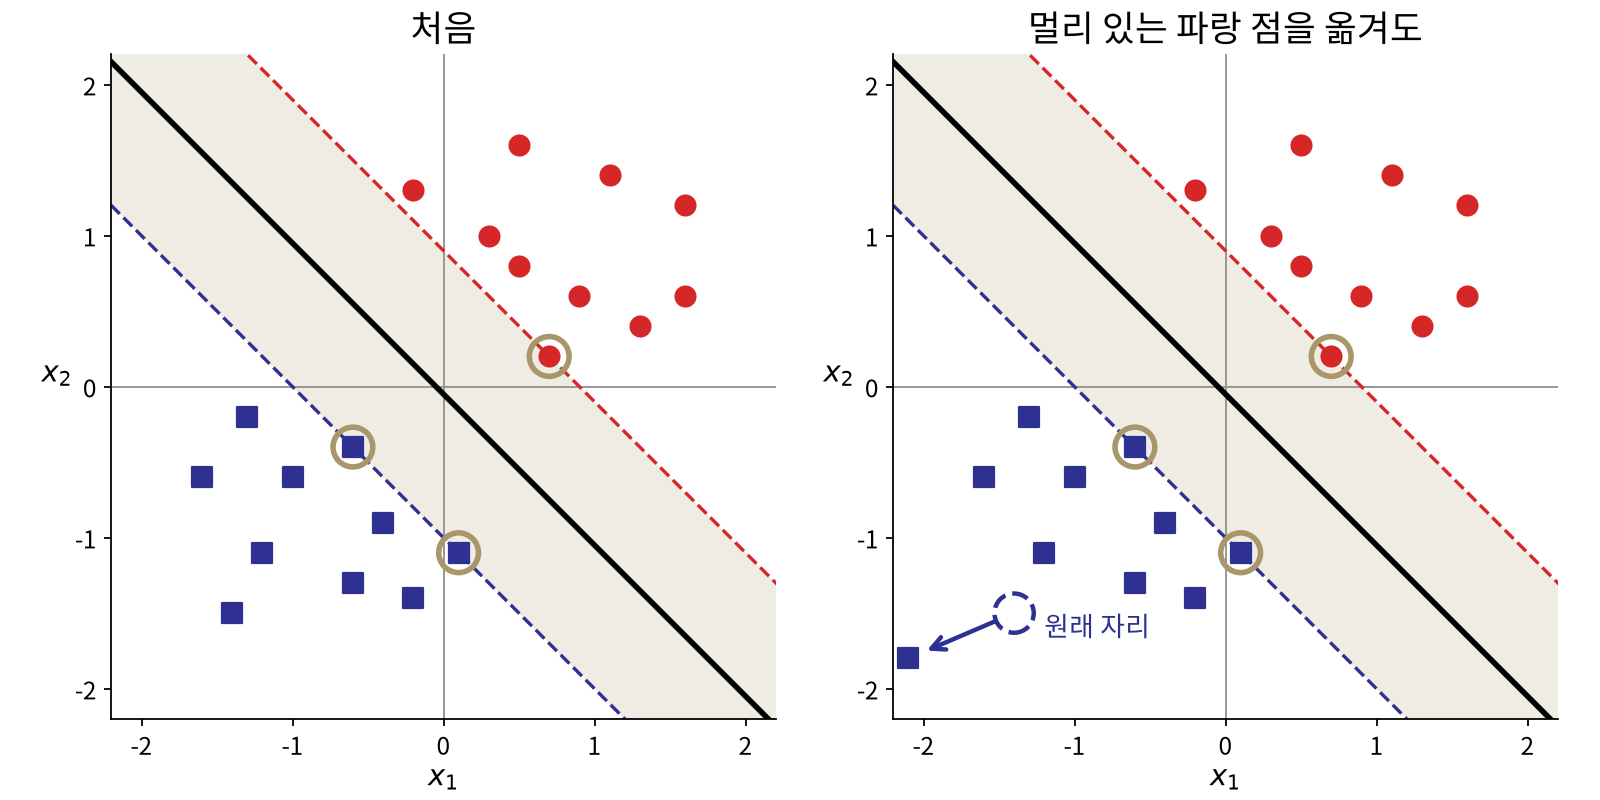
\includegraphics[width=0.62\linewidth]{sv_move.png}\par\vskip0.2em
{\large 먼 점은 옮겨도 경계가 \kq{그대로}}
\vfill
\note{이 경계는 20개 점 중 단 3개, 서포트 벡터가 정합니다. 빨강 하나, 파랑 둘입니다. 길 가장자리에서 멀리 떨어진 점은 경계에 아무 영향이 없습니다. 오른쪽 그림에서 왼쪽 아래의 파란 점 하나를 더 멀리 옮겼는데, 경계와 길은 그대로입니다. 반대로 서포트 벡터 하나를 옮기면 경계가 바뀝니다. 로지스틱회귀는 모든 점이 조금씩 경계에 영향을 주는 것과 대조적입니다.}
\end{frame}

% --- 왜 2~3개로 정해지나
\begin{frame}{왜 점 2$\sim$3개로 정해지나: 닿을 때까지 넓힌다}
\vfill
\centering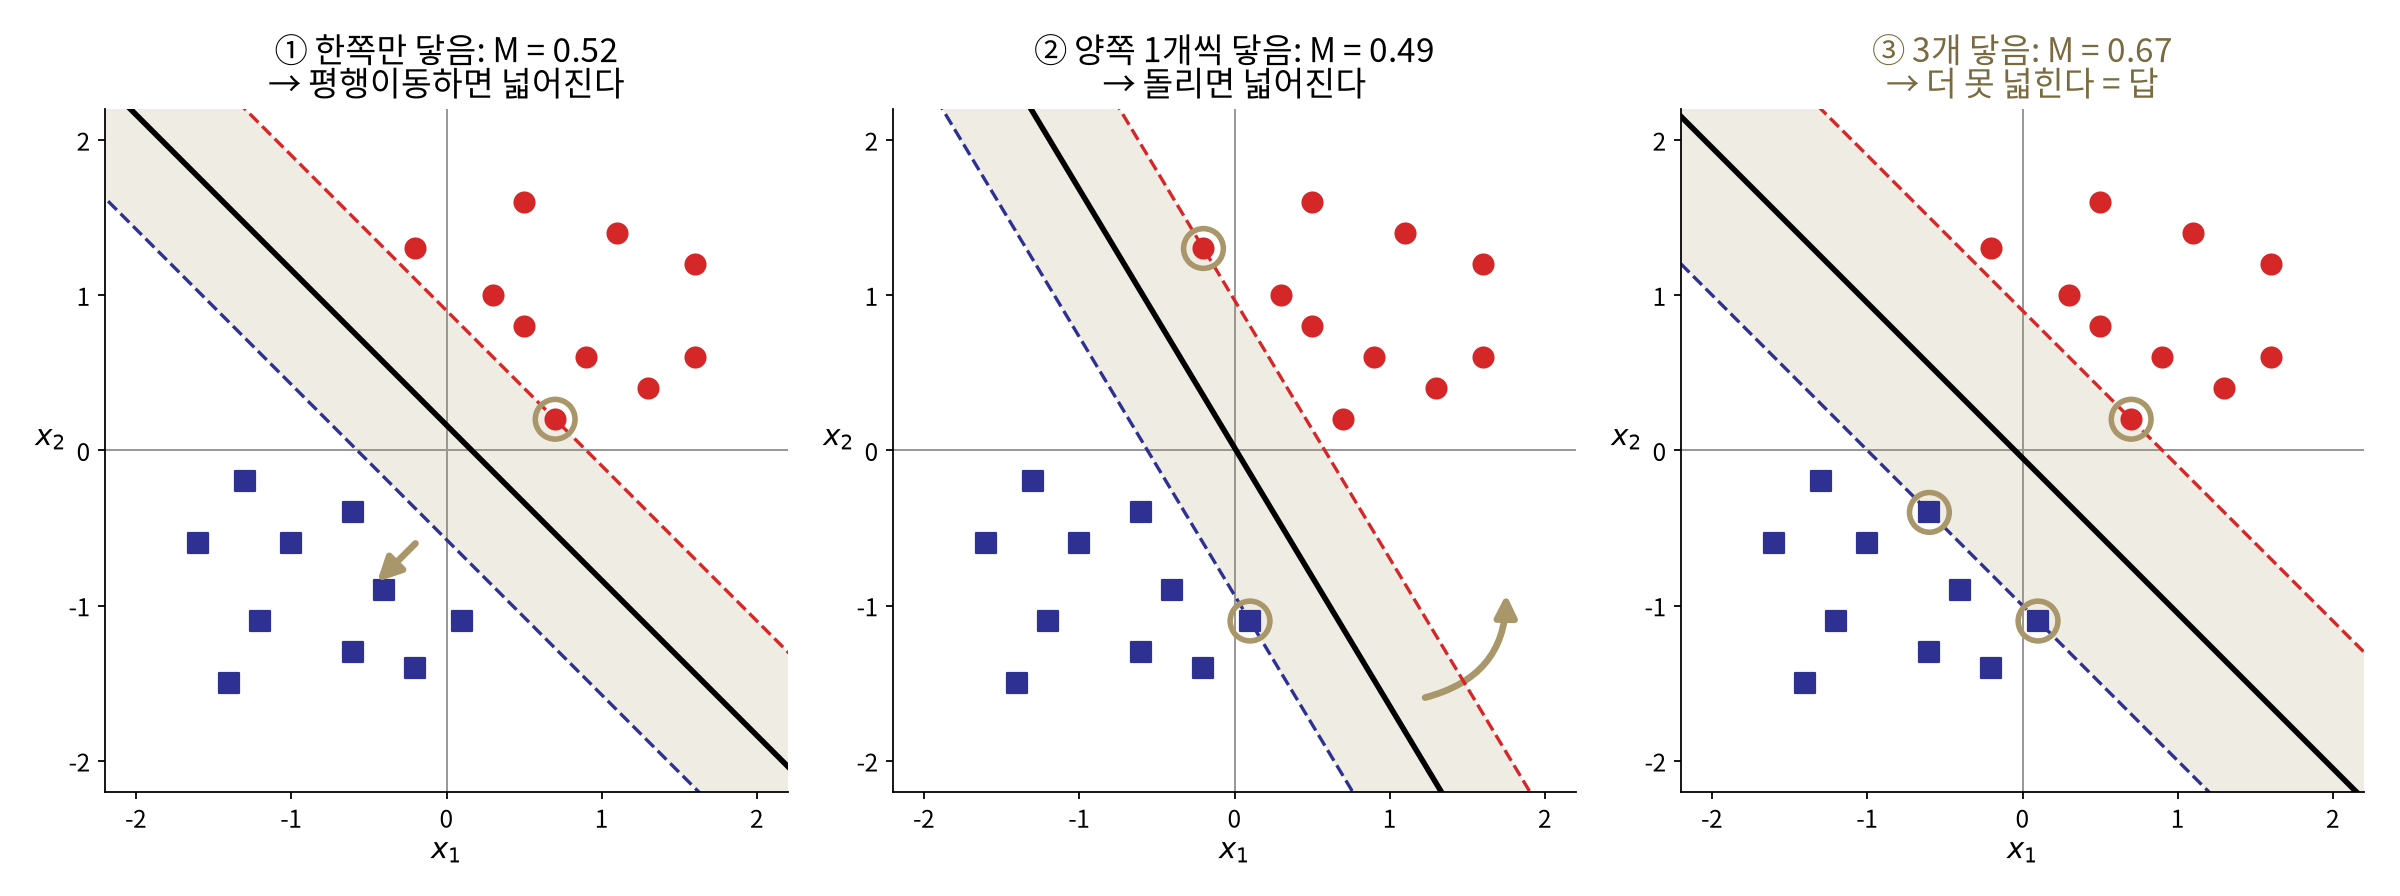
\includegraphics[width=0.94\linewidth]{sv_lock.png}\par\vskip0.2em
{\large 정할 것 3개 (기울기 · 위치 · $M$) $=$ 가장자리에 닿는 점 \kb{3개}}
\vfill
\note{왜 경계가 점 두세 개로 정해지는지 봅시다. 길을 최대로 넓혔다면 어떤 모양이어야 할까요. 첫째 그림처럼 한쪽, 빨강만 가장자리에 닿아 있으면 선을 파랑 쪽으로 평행이동하면 길이 넓어집니다. 그러니 최대가 아닙니다. 양쪽에 적어도 하나씩은 닿아야 합니다. 둘째 그림처럼 양쪽에 하나씩, 두 점만 닿아 있으면 선을 살짝 돌려서 두 점 모두에서 멀어질 수 있습니다. 예외는 선이 두 점을 잇는 선분에 수직일 때뿐이고, 그때는 두 점으로 끝납니다. 그 밖에는 돌리다 보면 세 번째 점이 닿아서 더 못 돌립니다. 셋째 그림이 그 상태, 우리 답입니다. 숫자로 보면 2차원에서 정할 것은 기울기, 위치, 그리고 M 세 개이고, 가장자리에 닿은 점 하나가 거리 = M이라는 식 하나를 주니 점 세 개면 딱 정해집니다. 특징이 n개면 보통 n 더하기 1개까지 닿습니다. 나머지 점은 M보다 멀어서 식에 들어가지 않고, 조금 움직여도 답이 바뀌지 않습니다.}
\end{frame}

% --- 2개 vs 3개
\begin{frame}{2개로 정해질 때 vs 3개로 정해질 때}
\vfill
\centering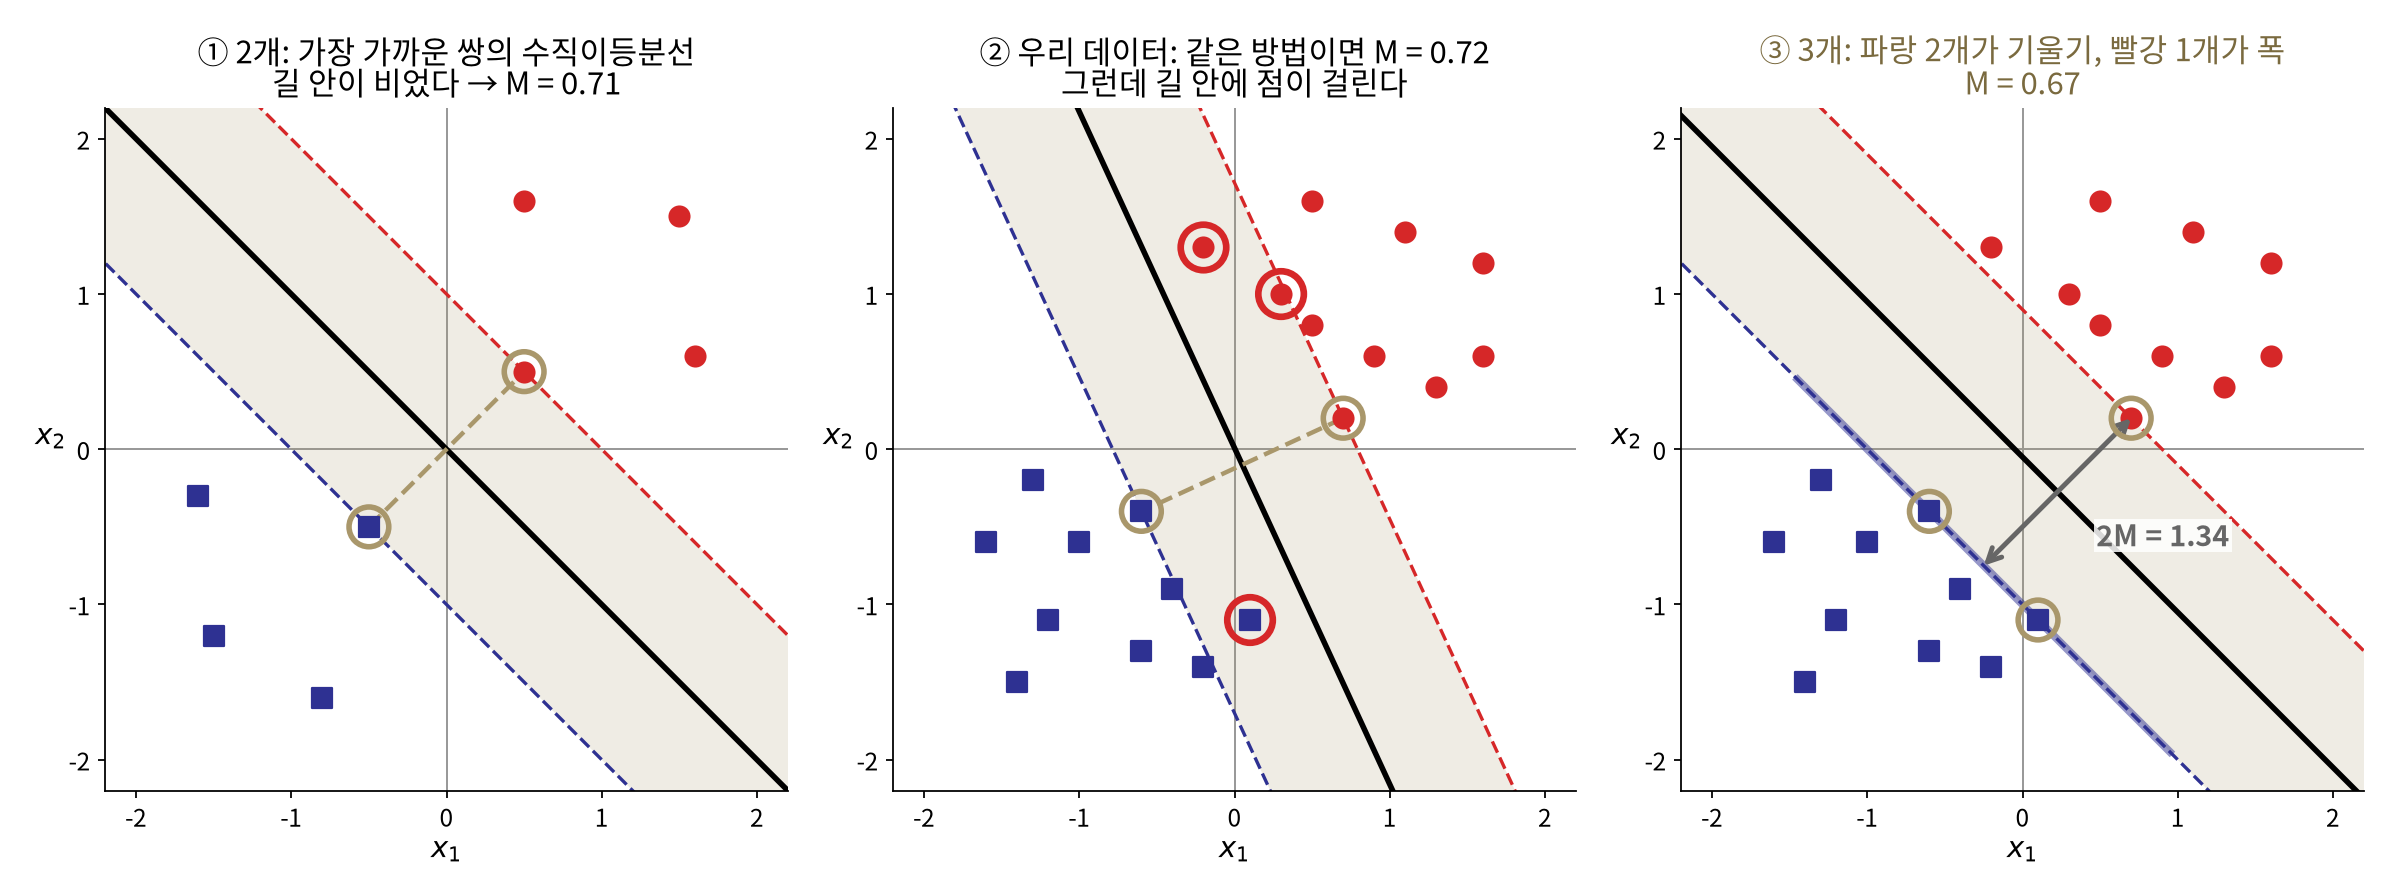
\includegraphics[width=0.94\linewidth]{sv_two_three.png}\par\vskip0.2em
{\large 가장 가까운 쌍의 수직이등분선 길이 \kb{비었으면 2개}, 점이 \kq{걸리면 3개}}
\vfill
\note{두 점으로 정해질 때와 세 점으로 정해질 때를 비교합니다. 왼쪽은 작은 예입니다. 빨강과 파랑 사이에서 가장 가까운 두 점을 잇고, 그 선분의 수직이등분선을 경계로 하면 M은 선분 길이의 절반, 0.71입니다. 이 길 안에 다른 점이 하나도 없으면 이것이 답이고, 두 점이 정합니다. 선이 두 점을 잇는 선분에 정확히 수직이라 어느 쪽으로 돌려도 한 점이 가까워지기 때문입니다. 가운데는 우리 데이터에 같은 방법을 쓴 것입니다. 가장 가까운 쌍은 빨강 0.7, 0.2와 파랑 마이너스 0.6, 마이너스 0.4이고 거리가 1.43이라 M은 0.72가 될 것 같지만, 그 길 안에 빨간 동그라미 점들이 걸립니다. 그래서 이 선은 쓸 수 없습니다. 오른쪽이 실제 답입니다. 파랑 두 점, 마이너스 0.6, 마이너스 0.4와 0.1, 마이너스 1.1을 이은 직선이 파랑 쪽 가장자리가 되어 기울기를 정합니다. 기울기가 정확히 마이너스 1이라 w가 0.71, 0.71입니다. 빨강 0.7, 0.2에서 그 직선까지의 거리 1.34가 길 폭 2M이 되어 폭을 정합니다. 그래서 M은 0.67로, 두 점으로 정할 때의 0.72보다 작습니다. 점이 많을수록 길 안에 점이 걸리기 쉬워서 세 점, 특징이 n개면 n 더하기 1개인 경우가 훨씬 흔합니다.}
\end{frame}

% --- 참고: 점곱과 코사인 (값 = 그림자 - 경계의 그림자 = 거리)
\begin{frame}{값에 $y_k$ 를 곱한다: 파랑 $D(\mathbf{x}) \to -D(\mathbf{x})$}
\vfill
\centering
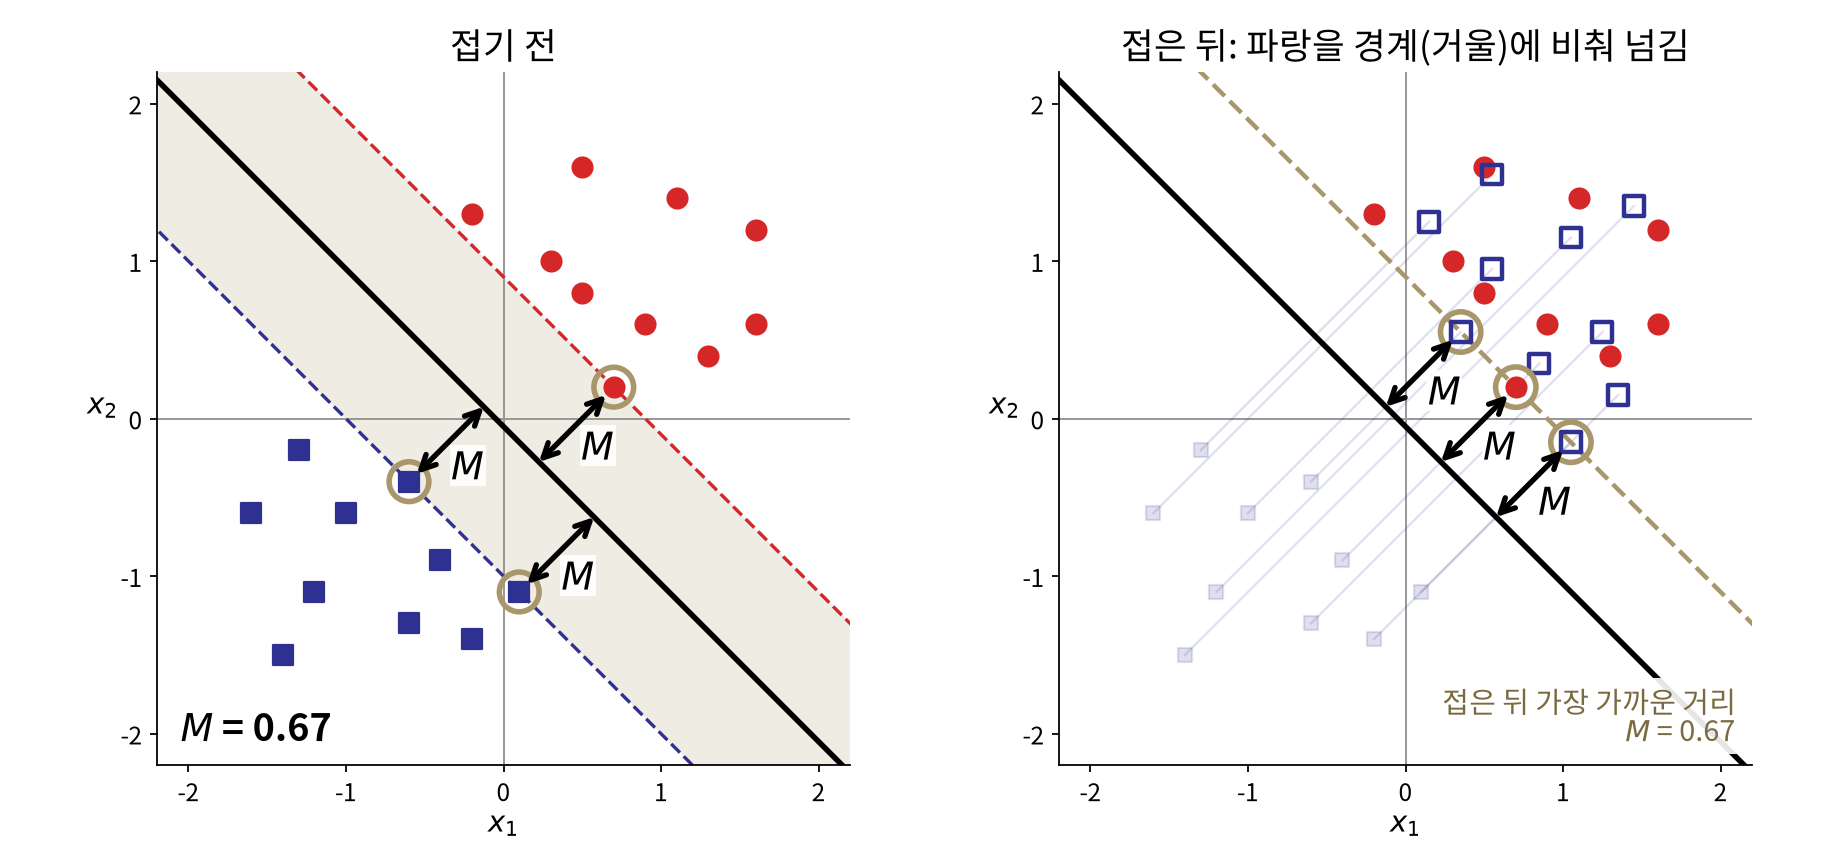
\includegraphics[width=0.68\textwidth]{sv_fold.png}\\[0.1em]
{\large 빨강 $D(\mathbf{x}_k)$, \; 파랑 $-D(\mathbf{x}_k)$ \;$\to$\; 둘 다 $y_k D(\mathbf{x}_k)$ = 거울까지 거리}\\[0.3em]
{\large 모든 점이 경계에서 $M$ 이상: \;$\dfrac{y_k D(\mathbf{x}_k)}{\lVert\mathbf{w}\rVert} \ge M$}
\vfill
\note{이번에는 점이 아니라 값, w 점곱 x 더하기 b에 y k를 곱합니다. 앞에서 점에 y k를 곱한 것, 원점 기준 180도 회전과는 다른 그림입니다. 파란 점은 y가 마이너스 1이라 값의 부호가 뒤집힙니다. 값은 경계까지의 거리이니, 부호만 뒤집힌 값을 갖는 자리는 경계 반대편으로 같은 거리, 즉 경계를 거울 삼아 비춘 자리입니다. 그래서 값에 y를 곱하는 것은 파란 점을 경계에 비춰 빨강 쪽으로 넘긴 것과 같습니다. 원점 기준으로 180도 돌리면 b가 0이 아닐 때 값이 달라집니다. 접고 나면 20개가 모두 한쪽에 있고, 각 점의 값은 거울까지의 거리입니다. 틀린 쪽에 있던 점이 있다면 접어도 거울 반대편에 남아 값이 음수가 됩니다. 빨강은 값 그대로, 파랑은 값에 마이너스를 붙이면 둘 다 거울까지의 거리가 되는데, 이 둘을 한 식으로 쓴 것이 y k 곱하기 D x k입니다. 그중 가장 작은 것이 M이고, 거울을 기울이고 옮겨서 이 M을 최대로 만드는 것이 바로 SVM, 최대 마진입니다. 뒤의 식 쪽에서 이 문장이 그대로 조건 y k D x k ≥ M이 됩니다. 답에서는 빨강 한 점과 비춰 넘긴 파랑 두 점이 똑같이 0.67 거리에 닿습니다. 거울을 움직이면 접힌 모양도 같이 바뀌니, 가장 가까운 점도 계속 바뀝니다.}
\end{frame}

\section{식}
% --- 최대 마진 식 해설 (말풍선)
\begin{frame}{최대 마진 초평면 찾기: 한 줄씩 읽기}
\vfill
\begin{minipage}{0.62\textwidth}
{\Large\begin{align*}
\text{find} \quad & w_1, w_2,\, b\\ & \text{that maximize } \tikzmarknode{mm}{M > 0}\\[0.4em]
\text{subject to} \quad & \tikzmarknode{nb}{w_1^2 + w_2^2 = 1},\\[0.4em]
& \tikzmarknode{cc}{y_k(w_1 x_{k1} + w_2 x_{k2} + b) \ge M}
\end{align*}}
\end{minipage}
\begin{tikzpicture}[remember picture,overlay]
\node[bub,anchor=west] (b1) at ([xshift=1.4cm,yshift=0.55cm]mm.east) {마진 $M$ 최대};
\draw[bubarr] (b1.west) -- (mm.east);
\node[bub,anchor=west] (b2) at ([xshift=1.4cm,yshift=-0.1cm]nb.east) {$\mathbf{w}$ 의 길이 $\lVert\mathbf{w}\rVert = \sqrt{w_1^2 + w_2^2}$ 를 1 로};
\draw[bubarr] (b2.west) -- (nb.east);
\node[bub,anchor=west] (b3) at ([xshift=0.6cm,yshift=-0.4cm]cc.east) {모든 점이 $M$ 이상};
\draw[bubarr] (b3.west) -- (cc.east);
\end{tikzpicture}
\vskip1.2em
\centering
{\large 이 데이터: \; $\mathbf{w} = (0.71,\ 0.71)$, \; $b = 0.04$, \; \kb{$M = 0.67$}}
\vfill
\note{한 줄씩 읽어 봅시다. 첫 줄, 마진 M을 최대로 합니다. 마진은 경계에서 가장 가까운 점까지의 거리입니다. 둘째 줄, w1 제곱 더하기 w2 제곱이 1, 즉 w의 L2 norm 제곱이 1, 길이 L2 norm을 1로 맞춥니다. b은 들어가지 않습니다. 그래야 식의 값이 곧 경계까지의 거리가 됩니다. 이 조건이 없으면 w를 두 배, 세 배 키우기만 해도 값이 커지니 M을 끝없이 키울 수 있어서 문제가 성립하지 않습니다. 점과 직선 사이 거리 공식에서 거리는 값의 절댓값을 w의 길이로 나눈 것이라, 길이를 1로 맞추면 값이 그대로 거리입니다. 이 공식이 왜 성립하는지는 앞의 참고 쪽에서 봤습니다. 셋째 줄, 모든 점에서 라벨 곱하기 값이 M 이상, 즉 모든 점이 자기 쪽으로 경계에서 M 이상 떨어져 있어야 합니다. 이 데이터의 답은 w가 0.71, 0.71, b가 0.04, M이 0.67입니다. 서포트 벡터 0.7, 0.2을 넣으면 값이 0.67, 딱 M입니다. 이 문제는 볼록 최적화라서 효율적으로 풀 수 있고 답이 하나로 정해집니다.}
\end{frame}

% --- 최대 마진 식 (공식 그대로, ISL 9.9-9.11)
\begin{frame}{최대 마진 초평면 찾기: Generalize ($n$ 개 특징, $p$ 개 점)}
\markpage{form}
\vfill
\centering
{\large\begin{align*}
\text{find} \quad & w_1, \dots, w_n,\, b\\ & \text{that maximize } M > 0\\
\text{subject to} \quad & \sum_{i=1}^{n} w_i^2 = 1,\\
& y_k(w_1 x_{k1} + w_2 x_{k2} + \cdots + w_n x_{kn} + b) \ge M \quad \text{for all } k = 1, \dots, p
\end{align*}}
{\large $y_k = +1$ (A) 또는 $-1$ (B)}

\vfill
\note{최대 마진 초평면을 찾는 문제를 원 논문, Boser, Guyon, Vapnik 1992년 논문의 식 9 그대로 쓰면 이렇습니다. 학습 데이터가 p개, 특징이 n개이고 라벨은 클래스 A면 플러스 1, B면 마이너스 1입니다. 점 번호는 k, 특징 번호는 i로 씁니다. w1부터 wn과 b, 그리고 마진 M을 골라서 M을 최대로 합니다. 조건은 두 가지입니다. w1부터 wn까지의 제곱합이 1, 그리고 모든 점에서 라벨 곱하기 초평면 식의 값이 M 이상. 앞 쪽에서 읽은 2차원 식을 특징이 n개인 경우로 그대로 늘린 것입니다.}
\end{frame}

\section{소프트 마진}
% --- 최대 마진의 약점
\begin{frame}{최대 마진의 약점: 겹치면 불가능, 점 하나에 민감}
\vfill
\centering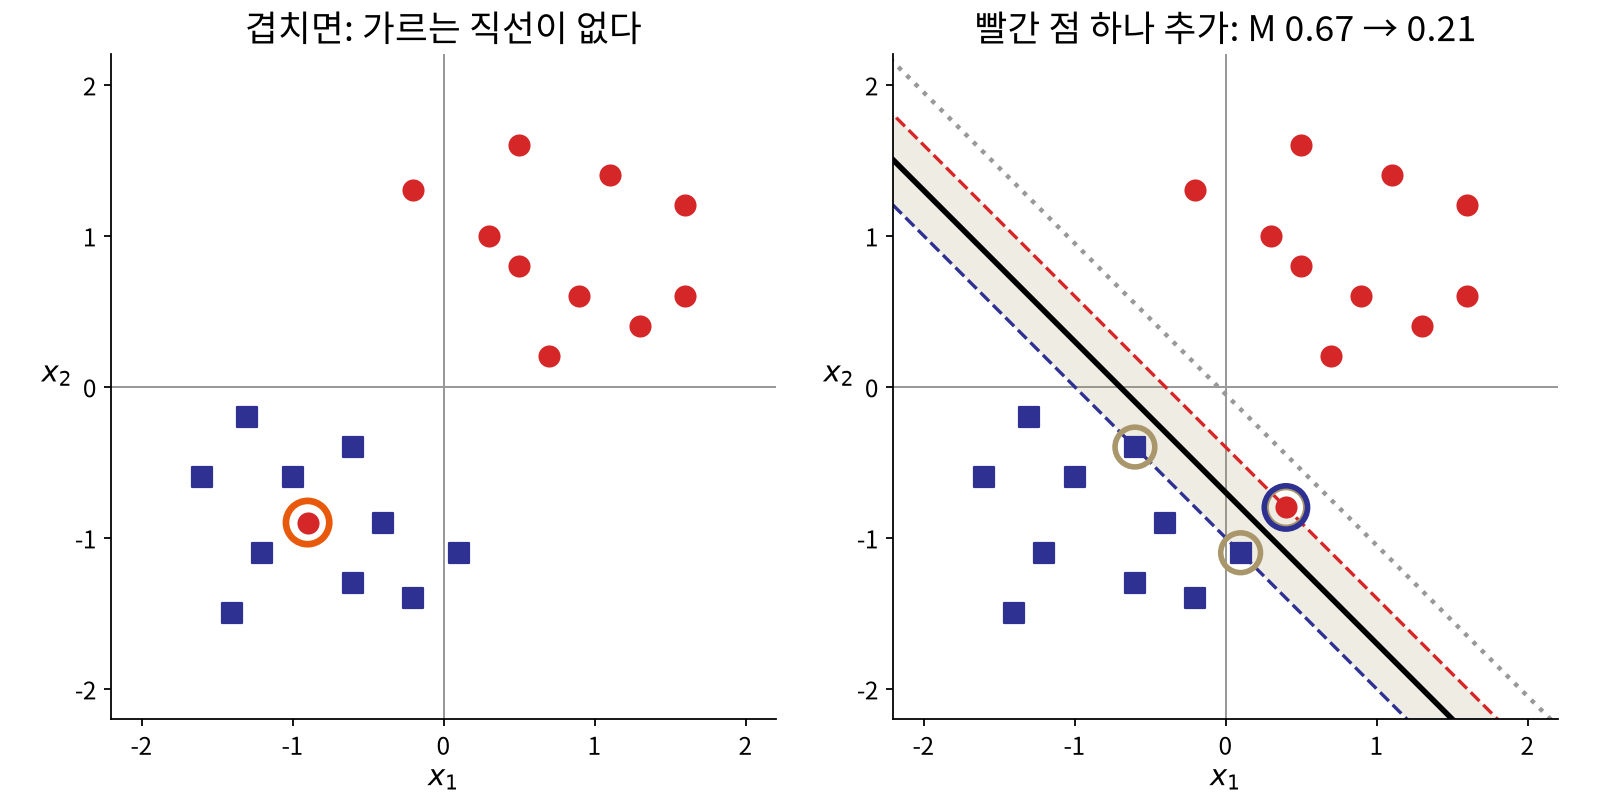
\includegraphics[width=0.66\linewidth]{../9_svm_extra/figs/sv_sensitive.png}\par\vskip0.2em
{\large 가를 수 \kq{없다} \quad 점 하나에 $M$ $0.67 \to 0.21$}
\vfill
\note{최대 마진 분류기에는 두 가지 약점이 있습니다. 첫째, 왼쪽처럼 빨간 점 하나가 파랑 무리 안에 들어오면 두 무리를 완벽히 가르는 직선이 아예 없습니다. 그러면 문제의 답이 없습니다. 둘째, 가를 수 있더라도 점 하나에 아주 민감합니다. 오른쪽은 빨간 점 하나를 0.4, 마이너스 0.8에 더한 것입니다. 마진이 0.67에서 0.21로 확 줄고, 경계도 점선이던 원래 경계에서 기울어집니다. 점 하나 때문에 경계가 크게 흔들리면 학습 데이터에 과대적합하기 쉽습니다.}
\end{frame}

% --- 서포트 벡터 분류기 식 (ISL 9.12-9.15, 최대 마진 식에 두 줄)
\begin{frame}{서포트 벡터 분류기 (소프트 마진) 찾기}
\markpage{soft}
\vfill
\hspace*{0.3cm}\begin{minipage}{0.6\textwidth}
{\large\begin{align*}
\text{find} \quad & \mathbf{w},\ b,\ \xi_1, \dots, \xi_p\\ & \text{that maximize } M > 0\\[0.2em]
\text{subject to} \quad & \lVert\mathbf{w}\rVert = 1,\\[0.2em]
& y_k D(\mathbf{x}_k) \ge \tikzmarknode{me}{M(1 - \xi_k)},\\[0.2em]
& \tikzmarknode{ep}{\xi_k \ge 0}, \quad \tikzmarknode{bb}{\textstyle\sum_{k} \xi_k \le B}
\end{align*}}
\end{minipage}
\begin{tikzpicture}[remember picture,overlay]
\node[bub,anchor=west] (s1) at ([xshift=0.8cm,yshift=0.5cm]me.east) {거리 $M$ 이상이거나,\\ 아니면 모자란 비율 $\xi_k$};
\draw[bubarr] (s1.west) -- (me.east);
\node[bub,anchor=east] (s2) at ([xshift=-1.4cm,yshift=-0.2cm]ep.west) {\textbf{슬랙 변수} $\xi_k$:\\ 점마다 하나};
\draw[bubarr] (s2.east) -- (ep.west);
\node[bub,anchor=west] (s3) at ([xshift=0.8cm,yshift=-0.3cm]bb.east) {넘어간 양의 \textbf{예산} $B$};
\draw[bubarr] (s3.west) -- (bb.east);
\end{tikzpicture}
\vskip1.6em
\centering{\large 최대 마진 식에서 \kb{$\ge M$} 이 \kq{$\ge M(1 - \xi_k)$} 로, 그리고 예산 한 줄}
\vfill
\note{깔끔하게 나뉘지 않을 때 쓰는 서포트 벡터 분류기, 소프트 마진의 식입니다. ISL 교과서와 스탠퍼드 강의가 쓰는 꼴이고, 앞에서 본 최대 마진 식에서 두 군데만 바뀝니다. 첫째, 조건의 오른쪽이 M이 아니라 M 곱하기 1 빼기 크사이 k입니다. 점마다 거리 M 이상이 원칙인데, 못 지키면 모자란 비율만큼 크사이를 씁니다. 이 크사이를 슬랙 변수라고 하고 점마다 하나씩 있습니다. 둘째, 크사이를 마음대로 쓰면 모든 점이 넘어가 버리니 크사이의 합이 예산 B를 넘지 못하게 묶습니다. 교과서는 이 예산을 C라고 쓰지만, sklearn의 C와 뜻이 반대라 헷갈리지 않게 여기서는 B라고 쓰겠습니다. 소프트 마진은 1995년 Cortes와 Vapnik의 논문, Support-vector networks에서 나왔고, SVM이라는 이름도 이 논문에서 나왔습니다.}
\end{frame}

% --- 슬랙 읽기
\begin{frame}{슬랙 $\xi_k$ 읽기: 넘어가도 되지만 예산 안에서}
\vfill
\begin{columns}[c]
\begin{column}{0.40\textwidth}\centering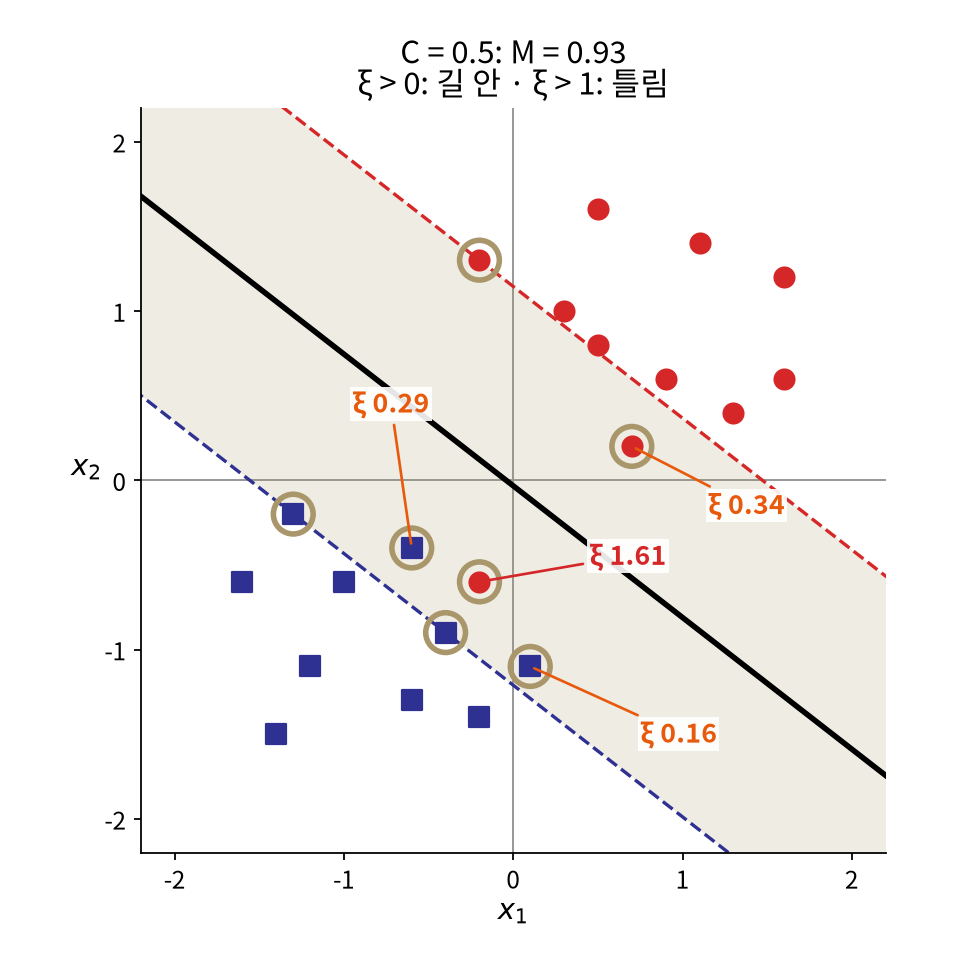
\includegraphics[width=0.95\linewidth]{../9_svm_extra/figs/sv_slack.png}\end{column}
\begin{column}{0.58\textwidth}
\renewcommand{\arraystretch}{1.3}
{\large\begin{tabular}{l|l}
$\xi_k = 0$ & 가장자리 바깥, 제자리\\
$0 < \xi_k \le 1$ & 가장자리를 넘어 길 안\\
$\xi_k > 1$ & 경계도 넘음 = \kq{틀림}\\
$B$ & $\sum_k \xi_k$ 의 \kb{예산}
\end{tabular}}
\end{column}
\end{columns}
\vfill
\note{그림으로 크사이를 읽어 봅시다. 크사이는 거리 M에서 모자란 비율입니다. 크사이가 0이면 원래대로 가장자리 바깥, 0보다 크고 1 이하면 가장자리를 넘어 길 안, 1보다 크면 경계까지 넘어 틀리게 분류된 것입니다. 그림의 M은 0.93입니다. 파랑 무리 안의 빨간 점은 크사이 1.61로 1보다 커서 틀렸고, 나머지 세 점은 0.16에서 0.34만큼 길 안에 들어와 있습니다. 다 더하면 2.41, 이 그림은 예산 B를 2.41까지 쓴 답입니다. 서포트 벡터는 가장자리 위의 점과 가장자리를 넘은 점 모두입니다.}
\end{frame}

% --- 예산 B 와 sklearn 의 C
\begin{frame}{예산 $B$: 크면 넓은 길 \quad (sklearn 의 $C$ 는 \kq{반대})}
\vfill
\centering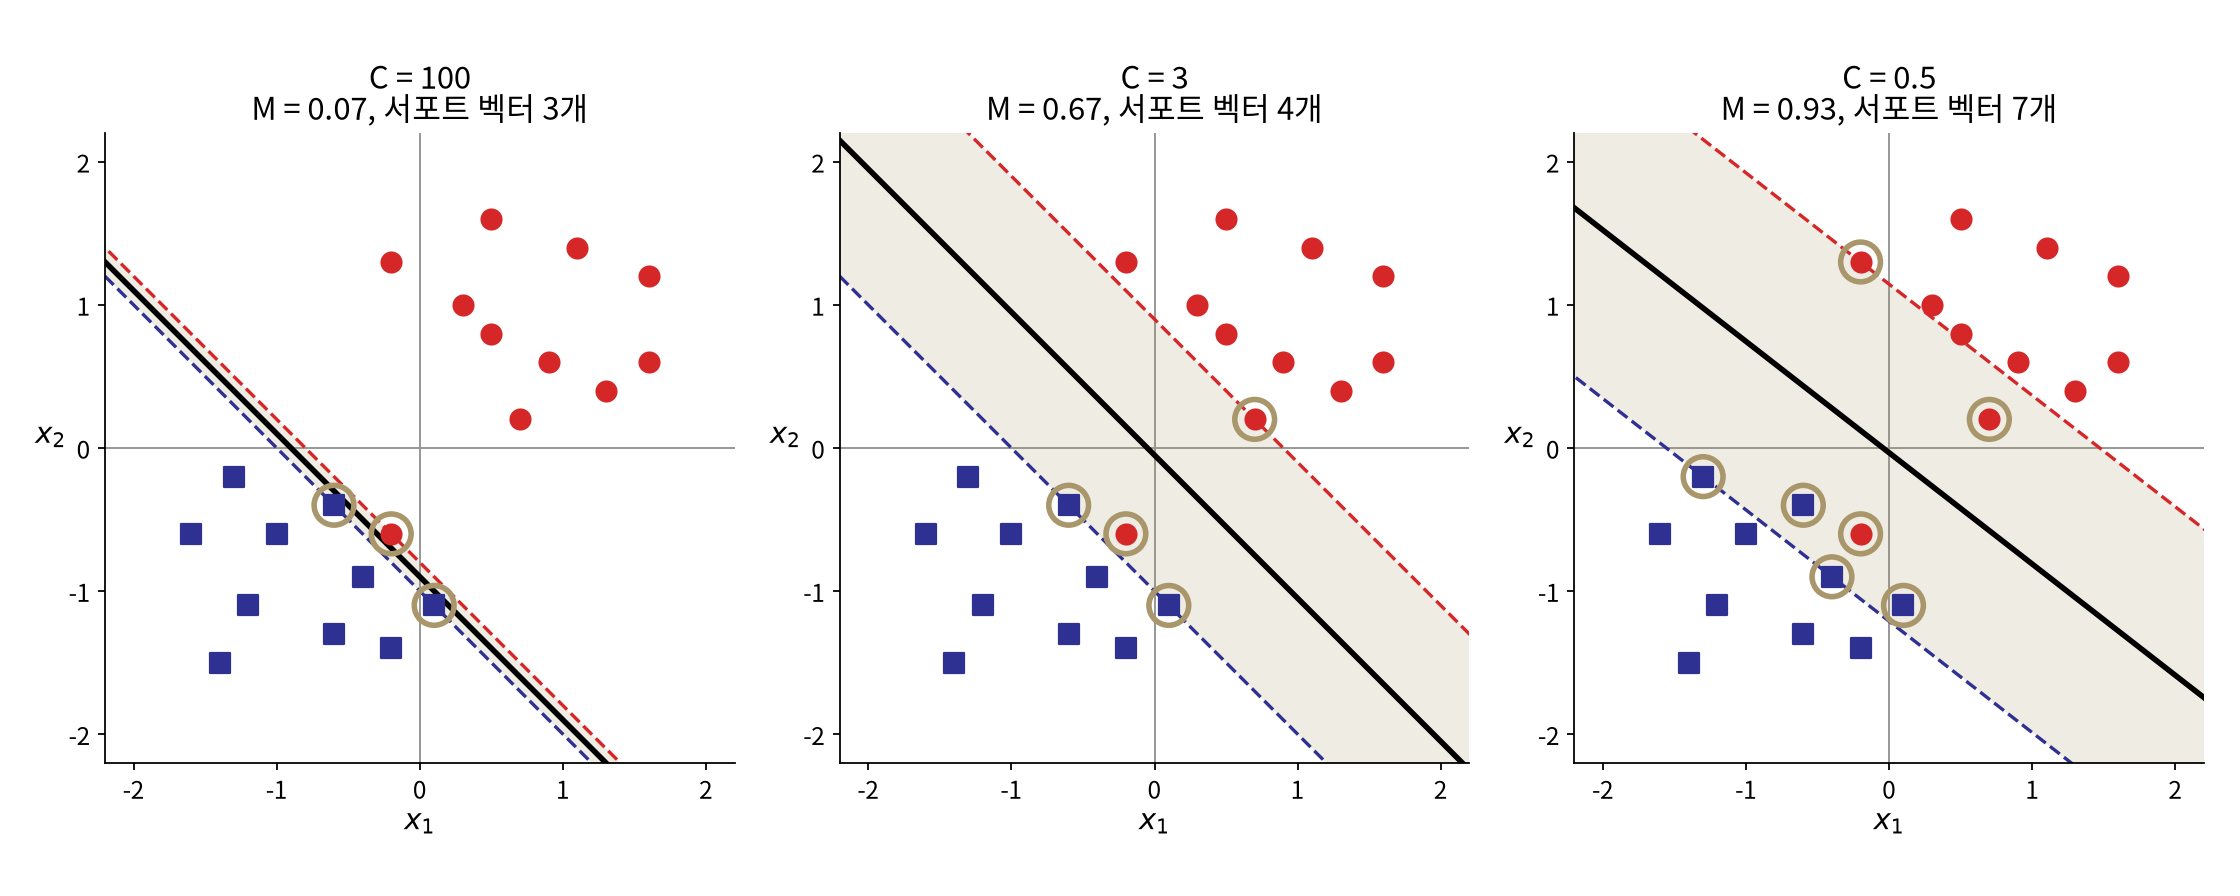
\includegraphics[width=0.56\linewidth]{../9_svm_extra/figs/sv_soft.png}\par\vskip0.2em
\renewcommand{\arraystretch}{1.25}
{\normalsize\begin{tabular}{r|ccc}
sklearn $C$ (넘어간 양의 \textbf{벌점}) & $100$ & $3$ & $0.5$\\ \hline
예산 $B = \sum_k \xi_k$ & $0$ & $1.79$ & $2.41$\\
마진 $M$ & $0.07$ & $0.67$ & $0.93$\\
서포트 벡터 & 3개 & 4개 & 7개
\end{tabular}}\\[0.4em]
{\normalsize $B$ \kb{크면} 넓은 길 $\cdot$ 서포트 벡터 많음 (편향 $\uparrow$, 분산 $\downarrow$) \quad $B$ 나 $C$ 는 \textbf{교차 검증}으로}
\vfill
\note{예산을 바꿔 봅시다. 실습에서 쓰는 sklearn은 예산 대신 넘어간 양에 거는 벌점 C를 받습니다. 벌점이 크면 넘어가기 싫으니 예산을 적게 쓰는 것과 같아서, 방향이 반대입니다. C가 100이면 이상치 하나까지 길 바깥에 두려고 길을 아주 좁혀 마진이 0.07, 넘어간 점이 없으니 예산 0, 서포트 벡터 3개입니다. C가 3이면 이상치 하나를 틀리게 두고 마진 0.67, 예산 1.79, 서포트 벡터 4개입니다. C가 0.5면 여러 점이 길 안에 들어오는 대신 마진이 0.93으로 넓어지고 예산 2.41, 서포트 벡터 7개입니다. 예산이 크면 경계가 여러 점의 영향을 고루 받아 덜 흔들리니 분산은 작고 편향은 큽니다. 예산이 0이면 최대 마진 분류기로 돌아갑니다. 예산이나 C는 교차 검증으로 고릅니다. C와 B 사이를 바로 바꾸는 간단한 공식은 없어서, 같은 선이 나오는 짝을 계산으로 찾았습니다.}
\end{frame}

\section{정리}
% --- 다중 클래스
\begin{frame}{클래스가 3개 이상이면}
\vfill
\centering
\renewcommand{\arraystretch}{1.6}
{\large\begin{tabular}{c|c|c}
 & {\Large\kb{일대일 (one-vs-one)}} & {\Large\kq{일대다 (one-vs-all)}}\\ \hline
만드는 법 & 클래스 두 개씩 짝마다 SVM & 클래스마다 ``나 vs 나머지'' SVM\\
개수 & $c(c-1)/2$ 개 & $c$ 개\\
예측 & \textbf{다수결} & $D$ 가 가장 큰 클래스\\ \hline
숫자 0$\sim$9 ($c = 10$) & \kb{45개} & \kq{10개}
\end{tabular}}
\vfill
\note{SVM은 초평면 하나로 두 쪽을 가르는 방법이라 기본은 두 클래스용입니다. 클래스가 c개면 두 가지 방법을 씁니다. 일대일은 클래스 두 개씩 짝을 지어 짝마다 SVM을 하나씩 만듭니다. c 곱하기 c 빼기 1 나누기 2개가 필요하고, 새 점은 모든 짝에서 이긴 클래스를 세어 가장 많이 이긴 클래스로 정합니다. sklearn의 SVC가 안에서 이 방식을 씁니다. 일대다는 클래스마다 나 대 나머지 전부로 SVM을 하나씩, 모두 c개 만들고, 새 점에서 D 값이 가장 큰, 즉 경계에서 가장 멀리 확신하는 클래스로 정합니다. 나머지 쪽이 훨씬 많아 불균형이 생길 수 있습니다. 손글씨 숫자 0부터 9까지면 일대일은 45개, 일대다는 10개입니다. SVM 원 논문의 손글씨 숫자 실험도 숫자마다 하나씩, 경계 10개를 만든 일대다였습니다.}
\end{frame}

\section{연습}
% --- 실습
\begin{frame}{실습}
\vfill
\centering\begin{tabular}{rl}
\large 1 & 슬라이드의 점 20개로 선형 SVM: $M$ 0.67 (폭 1.34), 서포트 벡터 3개, 먼 점 옮기기\\[0.5em]
\large 2 & 이상치 하나 넣고 소프트 마진: sklearn $C$ 에 따른 길 폭과 서포트 벡터 수
\end{tabular}\vskip1em
\href{https://colab.research.google.com/github/SuminHan/book-ml/blob/main/slides/ml1/week03/1_svm/lab/svm.ipynb}{\textcolor{ksagolddk}{▶ 1: 최대 마진 노트북}} \qquad
\href{https://colab.research.google.com/github/SuminHan/book-ml/blob/main/slides/ml1/week03/9_svm_extra/lab/svm_soft.ipynb}{\textcolor{ksagolddk}{▶ 2: 소프트 마진 노트북}}
\vfill
\note{실습은 두 부분입니다. 첫째, 슬라이드의 z-score 한 점 20개로 선형 SVM을 학습해서 마진 0.67, 길 폭 1.34와 서포트 벡터 3개를 재현하고, 먼 점을 옮겨도 경계가 그대로인지 확인합니다. 둘째, 빨간 이상치 하나를 파란 쪽에 넣고, sklearn의 C를 바꾸면 길 폭과 서포트 벡터 수가 어떻게 달라지는지 봅니다. C는 벌점이라 크면 좁은 길입니다. 커널과 지폐 데이터는 다음 시간 실습에서 합니다.}
\end{frame}

% --- 정리
\begin{frame}{정리}
\vfill
\centering\normalsize\begin{tabular}{l}
\textbf{초평면} $D(\mathbf{x}) = \mathbf{w}\cdot\mathbf{x} + b = 0$: 값의 부호로 양쪽을 나눈다\\[0.6em]
\textbf{최대 마진}: $\lVert\mathbf{w}\rVert = 1$ 로 두고 가장 가까운 점까지의 거리 $M$ 을 최대로\\[0.6em]
\textbf{서포트 벡터}: 가장자리에 닿은 점 몇 개가 경계를 정한다\\[0.6em]
\textbf{소프트 마진}: 슬랙 $\xi_k$ 로 넘어가도 되게, 합은 예산 $B$ 이하 (sklearn $C$ 는 벌점, 방향 반대)\\[0.6em]
\textbf{다중 클래스}: 일대일 $c(c-1)/2$ 개 · 일대다 $c$ 개\\[0.6em]
\kq{다음}: 직선으로 못 가르면? $\to$ 커널
\end{tabular}
\vfill
\note{정리합니다. 초평면은 값의 부호로 공간을 둘로 나눕니다. 최대 마진 분류기는 w의 길이를 1로 두고, 가장 가까운 점까지의 거리 M을 최대로 하는 초평면입니다. 경계는 가장자리에 닿은 서포트 벡터 몇 개가 정합니다. 점이 겹치면 슬랙 크사이로 가장자리나 경계를 넘어가는 것을 허락하되, 넘어간 양의 합을 예산 B 안으로 묶는 소프트 마진을 씁니다. sklearn은 같은 것을 벌점 C로 받아서 방향이 반대입니다. 클래스가 여러 개면 일대일이나 일대다로 SVM을 여러 개 씁니다. 다음 시간에는 직선으로 가를 수 없는 데이터를 커널로 다룹니다.}
\end{frame}

\begin{frame}{참고 문헌}
\vfill
\small
\begin{itemize}
\setlength{\itemsep}{0.7em}
\item Boser, B. E., Guyon, I. M., \& Vapnik, V. N. (1992). A training algorithm for optimal margin classifiers. \textit{COLT '92}, 144--152. \paperlink{https://doi.org/10.1145/130385.130401}
\item Cortes, C., \& Vapnik, V. (1995). Support-vector networks. \textit{Machine Learning}, 20(3), 273--297. \paperlink{https://doi.org/10.1007/BF00994018}
\item James, G., Witten, D., Hastie, T., \& Tibshirani, R. \textit{An Introduction to Statistical Learning}, 9장. \paperlink{https://doi.org/10.1007/978-1-0716-1418-1}
\item Wang, S. (2019). CME 250 Lecture 5: Support Vector Machines, Stanford. \paperlink{https://web.stanford.edu/class/cme250/files/cme250_lecture5.pdf}
\end{itemize}
\vfill
\note{이 덱의 참고 문헌입니다.}
\end{frame}
\end{document}
